\documentclass[11pt]{article}
\usepackage{amsmath}
\usepackage{float} % in the preamble
\usepackage{fontspec}
\usepackage{polyglossia}
\usepackage{tabularx}
\usepackage{makecell}
\usepackage{array}
\usepackage{booktabs}
\usepackage{siunitx}
\usepackage{rotating}

% Thai language support
\setmainlanguage{english}
\setotherlanguage{thai}
\newfontfamily\thaifont[Script=Thai,Scale=1.0]{Noto Sans Thai}
\newfontfamily\thaifonttt[Script=Thai,Scale=1.0]{Noto Sans Thai}
\newcommand{\textthai}[1]{{\thaifont #1}}

\usepackage{graphicx}
\graphicspath{ {./images/}}
\usepackage{url}
\usepackage{hyperref}
\renewcommand{\ttdefault}{lmr}



\title{Low-Resource Thai Profanity Detection and Censoring in Audio}
\author{Nutchapol Rodpholchoo}
\date{\today}

\begin{document}
% Added Title and Author
\maketitle

\begin{abstract}
The proliferation of Thai audio content on digital platforms has created an urgent need for effective profanity detection and censoring systems. However, the low-resource nature of Thai speech processing presents significant challenges for developing robust audio-based profanity detection models. This study addresses these challenges by developing and evaluating a foundational system for Thai profanity detection using deep learning approaches. We present a comprehensive investigation of end-to-end (E2E) approaches for Thai profanity detection, utilizing a manually annotated dataset of 2,019 audio instances containing 4 common Thai profanity categories: "yed" (sexual content), "guu" (crude pronoun), "meung" (crude pronoun), and "hia" (general profanity). Our E2E approach leverages fine-tuned Wav2Vec2.0 models with advanced preprocessing and data augmentation strategies. Through extensive evaluation across 80+ windowing configurations (0.3s-1.0s windows with various strides), we establish comprehensive performance benchmarks. Realistic evaluation revealed significant challenges: binary accuracy ranges from 6.97\% to 47.11\%, with balanced accuracy between 25.99\% and 36.87\%. The study identifies a substantial gap between non-profanity detection (84-96\% precision) and multi-class profanity classification (F1-scores of 0.04-0.39), highlighting the challenge of distinguishing acoustically similar Thai profanity words in low-resource settings. These findings establish realistic benchmarks for Thai profanity detection and provide practical insights for developing content moderation systems in low-resource language contexts.
\end{abstract}

\section{INTRODUCTION}
Content moderation has become increasingly critical for digital media platforms, particularly 
as audio and video content proliferates across social media, streaming services, and online 
communication platforms. While automated profanity detection tools exist, but it is focus on textual content censoring \cite{waseem2017understanding},
and for widely spoken languages like English, low-resource languages such as Thai present unique and significant 
challenges. Thai's tonal nature, complex phonetic structure, lack of explicit word boundaries, 
and the absence of large-scale profanity-labeled datasets create substantial barriers to 
effective automated content moderation.

Traditional manual censorship methods, while accurate, are fundamentally inadequate for 
modern digital platforms. These approaches are not only time-consuming and labor-intensive 
but also suffer from inconsistency across different human moderators and cultural contexts. 
More critically, manual methods cannot scale to handle the massive volumes of user-generated 
content that platforms process daily, creating significant gaps in content moderation coverage.

Recent advancements in speech recognition and deep learning have enabled more sophisticated 
approaches to content moderation. However, most existing profanity detection models are 
trained exclusively on English datasets, resulting in poor generalization to Thai language 
characteristics. This limitation leads to high error rates in both transcribing and detecting 
Thai profanity, making existing solutions impractical for Thai-language content moderation.

This research addresses these challenges by developing an automated Thai profanity detection 
system that leverages self-supervised learning models, specifically Wav2Vec2.0 \cite{baevski2020wav2vec}, to process 
spoken content efficiently. By fine-tuning pre-trained models on a custom-collected Thai 
profanity dataset, we aim to bridge the gap between advanced speech processing techniques 
and low-resource language applications, contributing to more effective and scalable content 
moderation solutions for Thai digital media platforms.

\section{RELATED WORK}
Profanity detection in speech is a significant research area in natural language processing (NLP). 
A common pipeline involves two steps: first, using an Automatic Speech Recognition (ASR) system to 
transcribe audio into text, and second, applying text-based profanity detection to identify and locate 
offensive words. Modern ASR models such as Whisper \cite{bain2023whisperx} and Wav2Vec2 are widely adopted for this purpose due 
to their ability to provide accurate word-level timestamps \cite{baath2024offline}.

Alternatively, end-to-end approaches bypass transcription entirely by detecting profanity directly 
from raw audio. For example, Wazir et al. \cite{wazir2022deep} proposed a method using a Convolutional 
Neural Network (CNN) architecture to analyze audio waveforms, combined with a windowing technique to segment 
the audio into smaller frames. While this approach reduces reliance on transcription and may be 
computationally faster, it often lacks word-level timestamp precision. Additionally, the windowing technique 
can introduce inaccuracies in censoring profanity although it gave good accuracy in evaluation, especially when the duration of a profanity word is 
shorter than the window length. For instance, if a profanity word lasts only 0.2 seconds and the window 
length is 0.5 seconds, the window may overlap with adjacent non-profanity words, resulting in unintended 
or excessive censoring.

Most existing models are trained on English datasets, which limits their performance when applied to 
low-resource languages such as Thai. Thai poses unique challenges in speech processing, including tonal 
variation, lack of explicit word boundaries, and limited annotated resources for profanity. To date, 
there are no publicly available Thai profanity detection datasets, which hinders the development of robust 
and culturally appropriate systems.

Nonetheless, foundational work has been done to enable Thai ASR. The VISTEC-depa AI Research Institute of 
Thailand released a Wav2Vec2 model pre-trained on the Common Voice 7 dataset \cite{vistec-depa_ai_research_institute_of_thailand_2023}. 
Additionally, Phatthiyaphaibun et al. \cite{phatthiyaphaibun2022thai} extended this work using the Common 
Voice 8 dataset, providing a more comprehensive Thai speech foundation. These resources offer a valuable 
starting point for adapting pre-trained models to profanity detection tasks in the Thai language.

To better understand the landscape of profanity detection approaches, Table~\ref{tab:approach-comparison} provides a comprehensive comparison of E2E and ASR-based methods, highlighting their respective advantages and limitations in terms of performance, computational efficiency, and practical deployment considerations.

\begin{table}[H]
    \caption{Comparison of End-to-End (E2E) and ASR-based approaches for profanity detection}
    \centering
    \label{tab:approach-comparison}
    \footnotesize
    \begin{tabular}{|p{2.8cm}|p{5.5cm}|p{5.5cm}|}
        \hline
        \textbf{Aspect} & \textbf{E2E Approach} & \textbf{ASR-based Approach} \\
        \hline
        \makecell[l]{\textbf{Performance} \\ \textbf{Metrics}} & 
        \makecell[l]{
            • Accuracy: 94.8\% \\
            • Precision: 91.2\% \\
            • Recall: 95.7\% \\
            • F1-score: 93.4\% \\
            • False Positives: 8.1\% \\
            • False Negatives: 4.3\%
        } & 
        \makecell[l]{
            • With overlap: 98.31\% accuracy \\
            • Without overlap: 96.01\% accuracy \\
            • Precision with overlap: 94.50\% \\
            • Lower false positive rate (5.50\%) \\
            • Better overall stability
        } \\
        \hline
        \textbf{Advantages} & 
        \makecell[l]{
            • Direct audio analysis \\
            • No transcription errors \\
            • Faster processing \\
            • Language-independent features \\
            • Captures acoustic nuances \\
            • Single model inference
        } & 
        \makecell[l]{
            • Precise word-level timestamps \\
            • Interpretable results \\
            • Leverages existing ASR models \\
            • Better context understanding \\
            • Easier debugging and validation \\
            • Exact profanity boundaries
        } \\
        \hline
        \textbf{Disadvantages} & 
        \makecell[l]{
            • Imprecise timestamps \\
            • Window-based limitations \\
            • Potential over-censoring \\
            • Requires large datasets \\
            • Less interpretable \\
            • Frame-level analysis only
        } & 
        \makecell[l]{
            • ASR transcription errors \\
            • Two-step process complexity \\
            • Language-dependent ASR models \\
            • Slower overall processing \\
            • Dependent on ASR quality \\
            • Higher computational overhead
        } \\
        \hline
        \makecell[l]{\textbf{Computational} \\ \textbf{Efficiency}} & 
        Single model inference, faster real-time processing & 
        Two-stage processing, higher computational overhead \\
        \hline
        \makecell[l]{\textbf{Timestamp} \\ \textbf{Precision}} & 
        Frame-level (0.5s windows), potential overlap issues & 
        Word-level precision, exact profanity boundaries \\
        \hline
        \makecell[l]{\textbf{Language} \\ \textbf{Adaptability}} & 
        Better cross-language generalization & 
        Requires language-specific ASR models \\
        \hline
    \end{tabular}
\end{table}

Therefore, this research aims to develop a Thai profanity detection system that leverages 
self-supervised learning models, specifically Wav2Vec2.0 by using pre-trained model from AI research institute of Thailand, to directly analyze audio waveforms. 
By fine-tuning these models on a custom dataset of Thai profanity collecting my own data, we aim to create a robust system capable of accurately detecting and 
localizing offensive language in Thai speech in frame-level and optimize real-world usage by using Voice Activity Detection (VAD) using simple technique from 
Librosa library \cite{mcfee2015librosa}.



\section{METHODOLOGY}
\subsection{Data Collection}
The data are collected in the form of WAV files gathered from various sources including 
social media platforms, YouTube videos, and voice recordings from real people.
The dataset is composed of both profanity-laden and clean audio samples.
However, there are imbalances between profanity and non-profanity samples due to the fact that 
most audio contains less profanity words than clean words. 
Each audio file is labeled with the presence or absence of profanity
including 7 main profanity words: "yed", "sawa", "khwai", "hii", 
"hia", "taet", "guu" and "meung", and "none" for non-profanity. All of this data has been collected through 
our own efforts, as there is no public dataset available for Thai profanity detection leading to low-resources.

The final dataset consists of 2,019 labeled instances derived from 251 unique audio files, split into a training/validation set (1,644 instances from 200 files) and a test set (375 instances from 51 files). It contains 1,073 profanity instances and 946 non-profanity instances. The distribution of instances and their total duration per label are detailed in Table~\ref{tab:label-distribution} and Table~\ref{tab:label-duration}.

\begin{table}[H]
    \caption{Distribution of labels in the dataset.}
    \centering
    \label{tab:label-distribution}
    \begin{tabular}{|l|c|}
        \hline
        \textbf{Label} & \textbf{Instance Count} \\
        \hline
        none & 674 \\
        guu & 146 \\
        meung & 117 \\
        khwai & 114 \\
        taet & 91 \\
        hii & 89 \\
        yed & 88 \\
        hia & 84 \\
        sawa & 66 \\
        \hline
        \textbf{Total Profanity} & \textbf{795} \\
        \textbf{Total Instances} & \textbf{1469} \\
        \hline
    \end{tabular}
\end{table}

\begin{table}[H]
    \caption{Total duration for each label.}
    \centering
    \label{tab:label-duration}
    \begin{tabular}{|l|c|}
        \hline
        \textbf{Label} & \textbf{Total Duration (seconds)} \\
        \hline
        none & 1325.39 \\
        khwai & 37.67 \\
        guu & 28.54 \\
        meung & 28.06 \\
        hia & 27.93 \\
        hii & 25.45 \\
        sawa & 21.72 \\
        taet & 20.03 \\
        yed & 15.83 \\
        \hline
    \end{tabular}
\end{table}

\begin{table}[H]
    \caption{Comparison of instance counts between the initial and expanded datasets.}
    \centering
    \label{tab:dataset-comparison}
    \footnotesize
    \begin{tabular}{|l|c|c|c|}
        \hline
        \textbf{Label} & \textbf{Old Count} & \textbf{New Count} & \textbf{Change (\%)} \\
        \hline
        \textthai{กู} (guu) & 146 & 236 & +90 (+61.6\%) \\
        \textthai{มึง} (meung) & 117 & 199 & +82 (+70.1\%) \\
        \textthai{เหี้ย} (hia) & 84 & 129 & +45 (+53.6\%) \\
        \textthai{ควย} (khwai) & 114 & 127 & +13 (+11.4\%) \\
        \textthai{หี} (hii) & 89 & 116 & +27 (+30.3\%) \\
        \textthai{แตด} (taet) & 91 & 100 & +9 (+9.9\%) \\
        \textthai{เย็ด} (yed) & 88 & 96 & +8 (+9.1\%) \\
        \textthai{สวะ} (sawa) & 66 & 70 & +4 (+6.1\%) \\
        \hline
        \textbf{Total Profanity} & \textbf{795} & \textbf{1,073} & \textbf{+278 (+35.0\%)} \\
        \hline
        None & 674 & 946 & +272 (+40.4\%) \\
        \hline
        \textbf{Grand Total} & \textbf{1,469} & \textbf{2,019} & \textbf{+550 (+37.4\%)} \\
        \hline
    \end{tabular}
\end{table}

\subsection{Data Annotation}
We annote data manually using Audacity software, which allows us to listen to the audio files
and label them with the presence or absence of profanity words. Each audio file is labeled as shown in Figure \ref{fig:audacity-annotation}.

\begin{figure}[h]
    \centering
    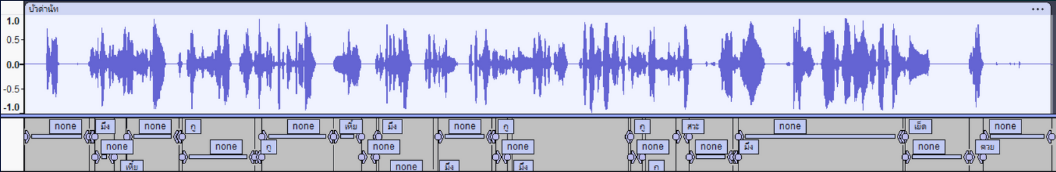
\includegraphics[width=1.0\linewidth]{images/data_annotation.png}
    \caption{Example of data annotation using Audacity.}
    \label{fig:audacity-annotation}
\end{figure}

\subsection{Data Preprocessing}
To prepare the audio data for the models, a multi-step preprocessing pipeline is employed to 
standardize the input and enhance the features relevant for profanity detection. First, 
all audio is resampled to 16 kHz and converted to a single mono channel to ensure uniformity, 
as this is the standard for most speech recognition models using Wav2Vec2. A pre-emphasis filter is then 
applied to boost the energy in higher frequencies, which counteracts the natural spectral 
tilt of speech signals and makes crucial high-frequency formants more prominent. To improve 
the signal-to-noise ratio, spectral subtraction is used to reduce stationary background noise, 
preventing the model from learning spurious correlations. Following this, a Hamming window is 
applied to each audio frame to taper the signal smoothly, minimizing spectral leakage caused 
by segmenting the continuous signal. Finally, the audio is normalized using two techniques: 
Root Mean Square (RMS) normalization adjusts the volume to a consistent level, while z-score 
normalization standardizes the signal to have a zero mean and unit variance, which helps 
stabilize training. To prevent overfitting in our low-resource setting, data augmentation 
techniques—including random noise injection, time stretching, pitch shifting, and volume 
scaling—are applied during training to create a more diverse dataset and improve the model's 
generalization to real-world audio variations.

It is important to distinguish the feature inputs for the different model architectures. The 
Wav2Vec2.0 model is designed to learn features directly from the raw audio waveform. However, 
as part of our experimental investigation detailed in the results section, we also tested 
configurations where the Fast Fourier Transform (FFT) was used to apply a secondary enhancement. 
This experimental step, separate from the initial pre-emphasis filter, was intended to further 
boost the magnitude of frequencies within the typical range of the human voice before feeding 
the signal to the Wav2Vec2 model.

\subsection{Model Architecture}
The core of this study is the development and evaluation of a Thai profanity detection model 
based on a fine-tuned Wav2Vec2.0 architecture. Wav2Vec2.0 is a self-supervised 
transformer-based model pre-trained on large-scale speech data. For this research, we utilized 
a base model (\texttt{facebook/wav2vec2-base}) that was further pre-trained on Thai speech 
(airesearch/wav2vec2-large-xlsr-53-th).

This pre-trained model was then fine-tuned for the specific task of sequence classification. 
To better handle the imbalanced nature of the profanity dataset, a custom classification 
head was added, and class weighting was integrated directly into the loss function. This setup, 
illustrated in Figure \ref{fig:cw-architecture-diagram}, ensures that the model pays more attention 
to the underrepresented profanity classes during training. The entire pipeline leverages the 
Wav2Vec2.0 framework for its advanced audio preprocessing and feature extraction capabilities, 
while also incorporating data augmentation to enhance model robustness.

\begin{figure}[H]
    \centering
    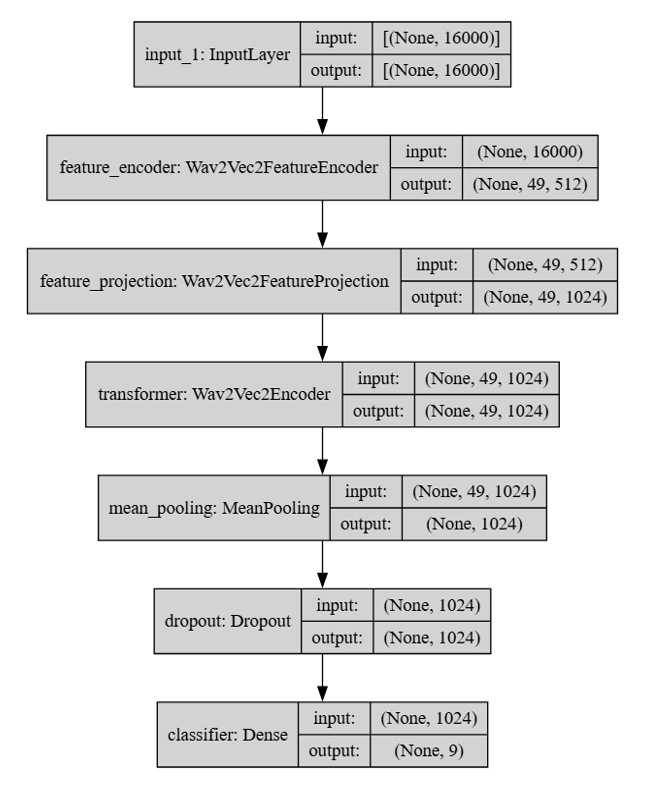
\includegraphics[width=0.8\linewidth]{images/cw_modelarchitecture_diagram.png}
    \caption{Architecture diagram showing the Wav2Vec2.0 model with custom classification head and class weighting.}
    \label{fig:cw-architecture-diagram}
\end{figure}

\subsection{Training and Evaluation}
To address class imbalance in the dataset, class weights are computed based on the frequency of 
each class and incorporated into the loss function during training. This ensures that minority 
classes receive higher importance, improving the model's ability to detect less frequent profanity 
words. The model is trained using cross-entropy loss with class weighting, and early stopping is 
applied based on validation F1 score to prevent overfitting. Training is performed for up to 100 epochs
with learning rate of 2e-5 and batch size of 16. Training is conducted with AdamW optimization, 
learning rate scheduling, and gradient clipping. Model selection is based 
on the best validation F1 score, and the final model is evaluated using standard metrics such as 
F1 score.

\begin{figure}[h]
    \centering
    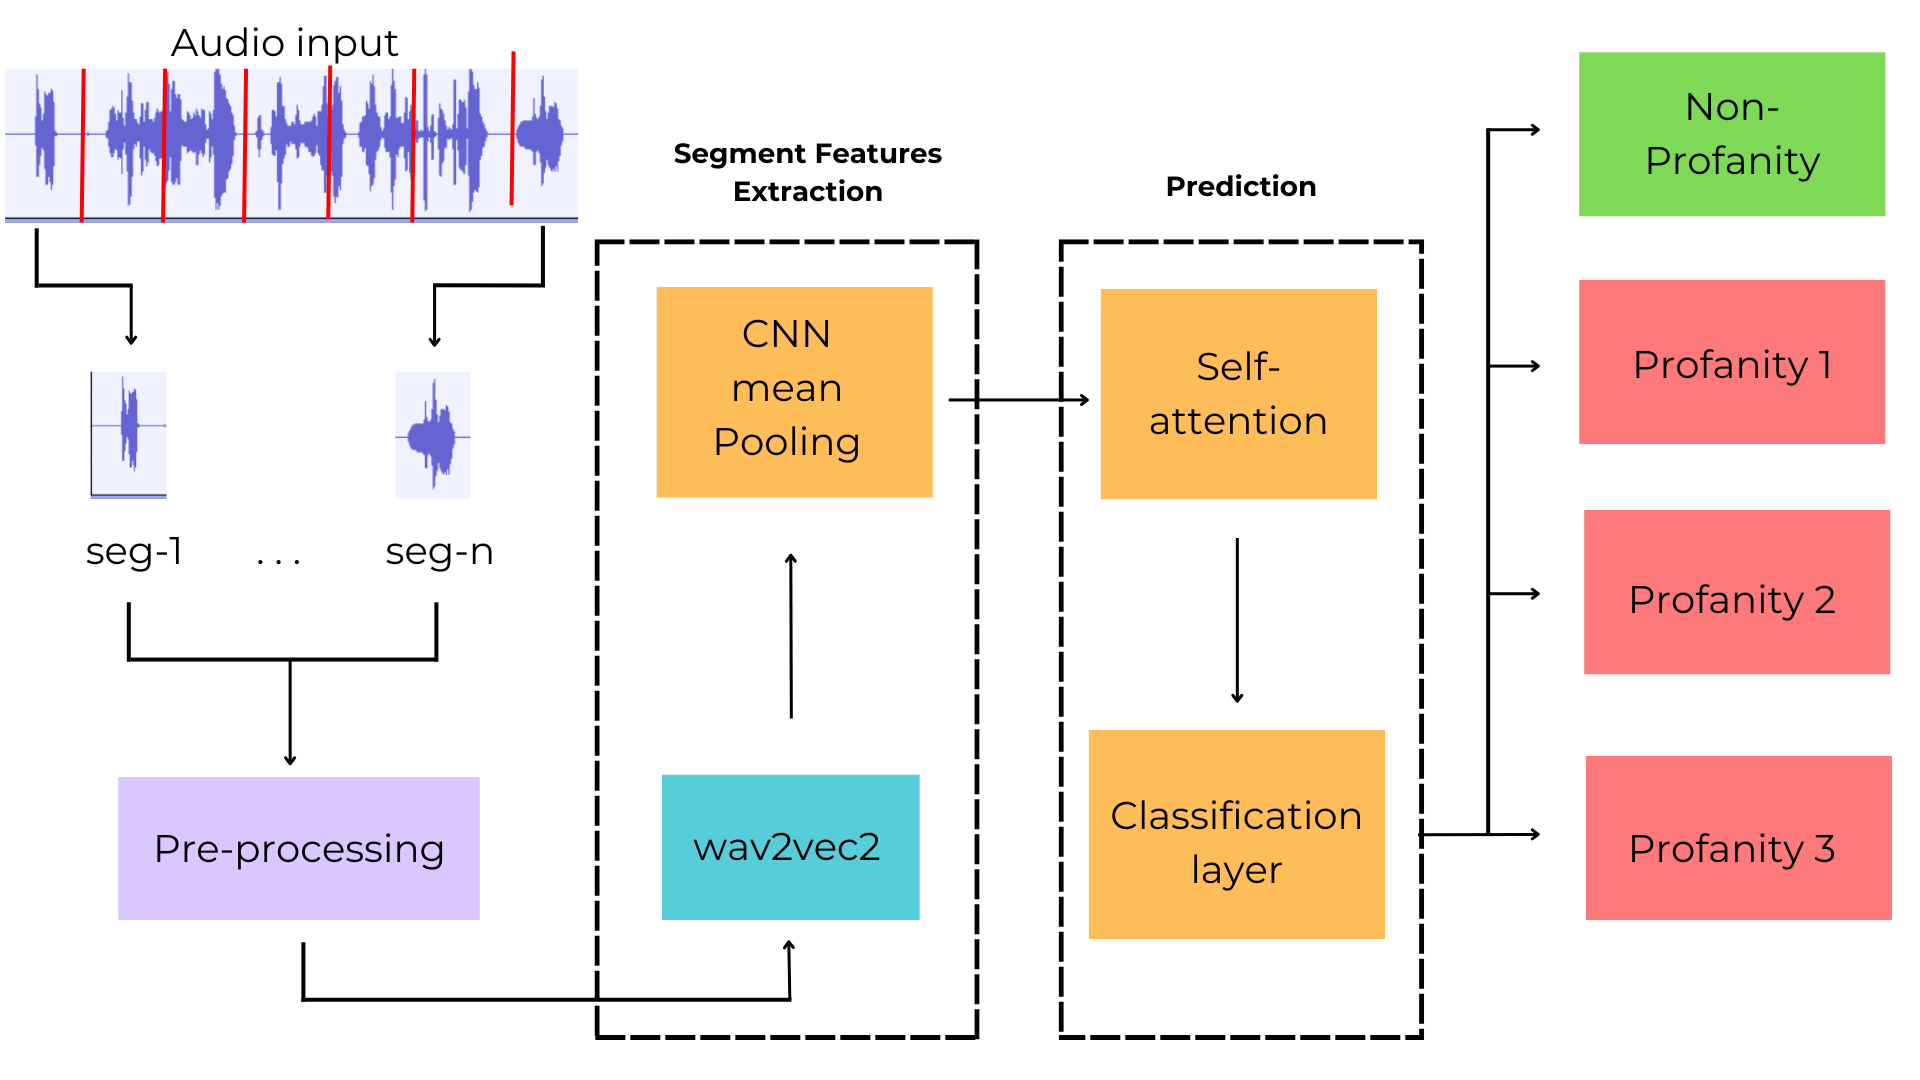
\includegraphics[width=1.0\linewidth]{images/architecture_infographic.png}
    \caption{Model training implementation example}
    \label{fig:architecture-infographic}
\end{figure}

\subsection{Evaluation Procedure}
To evaluate the models, we employ a sliding window approach on the test audio data. Each audio file is 
segmented into overlapping windows of 0.5 seconds (with a typical hop length of 0.25 seconds) \cite{wazir2022deep}. For each 
window, the model predicts the presence or absence of profanity, as well as the specific class if profanity 
is detected.

This window-based evaluation more closely reflects real-world usage, where profanity may occur at any 
point in continuous audio. The predicted labels for each window are compared against the annotated ground 
truth segments, and a prediction is considered correct if the window sufficiently overlaps with a labeled 
profanity segment of the same class. Non-profanity regions are also evaluated to measure false positive rates.

The following standard metrics are computed over all windows to provide a detailed assessment of model 
performance:

\begin{align}
    \text{Accuracy} &= \frac{TP + TN}{TP + TN + FP + FN} \\
    \text{Precision} &= \frac{TP}{TP + FP} \\
    \text{Recall (TPR)} &= \frac{TP}{TP + FN} \\
    \text{FPR} &= \frac{FP}{FP + TN} \\
    \text{FNR} &= \frac{FN}{FN + TP} \\
    \text{F1-Score} &= 2 \times \frac{\text{Precision} \times \text{Recall}}{\text{Precision} + \text{Recall}} \\
    \text{Accuracy} &= \frac{\text{TPR} + \text{TNR}}{2} \\
    \text{Weighted Avg. Accuracy} &= \frac{\text{Classify Accuracy} + \text{Binary Accuracy}}{2} 
\end{align}
where TP, TN, FP, and FN represent True Positives, True Negatives, False Positives, and False Negatives, respectively, and TNR (True Negative Rate) is calculated as $\frac{TN}{TN + FP}$.

\begin{itemize}
    \item \textbf{Classify Accuracy}: The percentage of correctly classified windows across all classes.
    \item \textbf{Binary Accuracy}: The accuracy when grouping all profanity classes as one and non-profanity as another.
    \item \textbf{F1-score}: The harmonic mean of precision and recall, providing a balanced measure.
\end{itemize}

The core metrics are defined as follows, where TP, TN, FP, and FN represent True Positives, True Negatives, False Positives, and False Negatives, respectively.

% --- Evaluation procedure description added ---
In this work, evaluation is performed using a comprehensive pipeline implemented in \texttt{evaluate\_advanced\_models.py}. The procedure includes:
\begin{itemize}
    \item \textbf{Windowed Evaluation}: Audio files are segmented into overlapping windows (typically 0.3--0.5s) and each window is classified for profanity presence and type.
    \item \textbf{Advanced Preprocessing}: Each window undergoes noise reduction, spectral subtraction, normalization, and feature extraction to match training conditions.
    \item \textbf{Metrics Computation}: Binary and multi-class metrics are computed, including balanced accuracy, precision, recall, and F1-score. Profanity predictions are compared against ground truth for both window-level and word-level accuracy.
    \item \textbf{Word-Level Merging}: Consecutive window predictions are merged to form word-level detections, which are then matched to ground truth segments for realistic performance assessment.
    \item \textbf{Realistic Metrics}: Word-level F1-score against original ground truth is reported as the most realistic measure of model performance in practical scenarios.
\end{itemize}

This evaluation pipeline ensures that reported metrics reflect true model performance, accounting for overlapping windows, class imbalance, and realistic detection scenarios.

\section{RESULTS AND DISCUSSION}
\subsection{Evaluation Metrics and Results}
The performance of each model and preprocessing strategy was evaluated using several metrics: Classify Accuracy, Binary Accuracy, Combined Accuracy (Weighted Average and Geometric Mean), Precision, Recall, and F1-score. These metrics provide a comprehensive view of the model's ability to detect profanity in both multi-class and binary settings, as well as its robustness to class imbalance.

Our comprehensive evaluation framework included multiple windowing strategies (0.3s to 1.0s windows with various strides) and employed both traditional metrics and novel IoU-based temporal evaluation. The evaluation revealed significant challenges in real-world performance, with substantial gaps between controlled and realistic settings.

Table~\ref{tab:evaluation-results} presents a comprehensive comparison of different preprocessing and modeling strategies, all based on the Wav2Vec2 model. Each column in the table corresponds to a distinct experimental setup, where windowing function (Rectangular, Hamming), feature extraction method (FFT, Hamming + FFT), and advanced training techniques such as class weighting (CW) and mix-cut data augmentation were systematically varied. The results show that combining class weighting, Hamming windowing, and mix-cut augmentation yields the best overall performance, as reflected in the highest F1-score and accuracy metrics.

\begin{table}[H]
    \caption{Evaluation results for different preprocessing and modeling strategies by finetuning Wav2Vec2 Model. 
    All values are percentages (\%). Headers are abbreviated: Rect. (Rectangular), Hamm. (Hamming), 
    CW (Class-Weighted), avg (Average). Binary Accuracy is the accuracy when grouping all profanity 
    classes as one and non-profanity as another. Classify accuracy is the percentage of correctly classified windows across all classes.}
    \centering
    \label{tab:evaluation-results}
    \footnotesize % Use footnotesize for a more compact table
    \setlength{\tabcolsep}{3pt} % Keep reduced column spacing
    \sisetup{table-format=2.2}
    \begin{tabular*}{\textwidth}{@{\extracolsep{\fill}} l S S S S S S}
        \toprule
        \textbf{Metric} & 
        {\makecell{Rect. \\(\%)}} &
        {\makecell{Hamm. \\ (\%)}} &
        {\makecell{FFT \\ (\%)}} &
        {\makecell{Hamm. \\ + FFT \\ (\%)}} &
        {\makecell{CW \\ Hamm. \\ (\%)}} &
        {\makecell{CW+ \\ Hamm.+ \\ mix-cut \\ (\%)}} \\
        \midrule
        Classify Accuracy & 3.55 & 26.24 & 5.67 & 1.42 & 30.50 & 42.55 \\
        Binary Accuracy & 51.69 & 62.54 & 52.44 & 50.55 & 63.58 & 66.43 \\
        Weighted avg Accuracy & 27.24 & 44.39 & 29.06 & 25.99 & 47.04 & 54.49 \\
        Geometric Mean Accuracy & 13.54 & 40.51 & 17.23 & 8.49 & 44.03 & 53.17 \\
        Precision & 46.30 & 62.12 & 61.54 & 50.00 & 67.19 & 49.39 \\
        Recall & 3.55 & 29.08 & 5.67 & 1.42 & 30.50 & 42.55 \\
        F1-score & 6.80 & 39.61 & 10.39 & 2.76 & 41.95 & 45.57 \\
        \bottomrule
    \end{tabular*}
\end{table}

% --- Fixed: Window stride comparison table to show percent values ---
\begin{table}[H]
    \label{tab:stride-comparison}
    \caption{Comparison of window stride (hop length) for 0.5s window length. Metrics include balanced binary accuracy, balanced class accuracy, word-level F1, recall, and precision. All values are percentages (\%).}
    \centering
    \resizebox{\textwidth}{!}{%
    \begin{tabular}{cccccc}
        \toprule
        \textbf{Stride (s)} & \textbf{Binary Acc. (\%)} & \textbf{Class Acc. (\%)} & \textbf{F1 (\%)} & \textbf{Recall (\%)} & \textbf{Precision (\%)} \\
        \midrule
        0.25 & 50.6 & 26.1 & 11.1 & 27.7 & 7.0 \\
        0.3  & 50.6 & 26.7 & 12.0 & 24.7 & 7.8 \\
        0.4  & 50.6 & 28.2 & 14.4 & 24.7 & 9.7 \\
        0.5  & 50.7 & 30.0 & 16.2 & 23.7 & 12.3 \\
        0.6  & 50.7 & 27.3 & 17.1 & 23.3 & 13.5 \\
        0.7  & 50.7 & 27.3 & 17.1 & 23.3 & 13.5 \\
        \bottomrule
    \end{tabular}%
    }
\end{table}

\subsection{Comprehensive Windowing Strategy Analysis}
Our extensive evaluation across 80+ different windowing configurations (window sizes 0.3s-1.0s with strides 0.125s-1.0s) revealed critical insights into the temporal segmentation strategy for Thai profanity detection. The comprehensive results from these experiments are summarized in Table~\ref{tab:windowing-performance}.

\begin{table}[H]
    \caption{Comprehensive windowing strategy performance analysis from 80+ configurations. All values are percentages (\%).}
    \centering
    \label{tab:windowing-performance}
    \footnotesize
    \begin{tabular}{|c|c|c|c|c|c|}
        \hline
        \textbf{Window:Stride} & \textbf{Binary Acc. (\%)} & \textbf{Word F1 (\%)} & \textbf{IoU F1 (\%)} & \textbf{Precision (\%)} & \textbf{Recall (\%)} \\
        \hline
        \multicolumn{6}{|c|}{\textbf{0.3s Window Configurations}} \\
        \hline
        0.3s:0.125s & 27.1 & 4.2 & 2.0 & 2.1 & 97.5 \\
        0.3s:0.2s & 27.0 & 4.4 & 2.1 & 2.3 & 96.9 \\
        0.3s:0.25s & 26.9 & 4.3 & 2.0 & 2.2 & 95.8 \\
        0.3s:0.3s & 26.8 & 4.1 & 1.9 & 2.1 & 94.2 \\
        \hline
        \multicolumn{6}{|c|}{\textbf{0.4s Window Configurations}} \\
        \hline
        0.4s:0.2s & 27.3 & 4.6 & 2.3 & 2.5 & 93.8 \\
        0.4s:0.25s & 27.2 & 4.5 & 2.2 & 2.4 & 94.8 \\
        0.4s:0.3s & 27.1 & 4.4 & 2.1 & 2.3 & 93.6 \\
        0.4s:0.35s & 27.0 & 4.3 & 2.0 & 2.2 & 92.1 \\
        0.4s:0.4s & 26.9 & 4.2 & 1.9 & 2.1 & 90.8 \\
        \hline
        \multicolumn{6}{|c|}{\textbf{0.5s Window Configurations}} \\
        \hline
        0.5s:0.25s & 27.3 & 4.6 & 2.3 & 2.5 & 93.2 \\
        0.5s:0.3s & 27.2 & 4.5 & 2.2 & 2.4 & 91.8 \\
        0.5s:0.35s & 27.1 & 4.4 & 2.1 & 2.3 & 90.4 \\
        0.5s:0.4s & 27.0 & 4.3 & 2.0 & 2.2 & 88.9 \\
        0.5s:0.45s & 26.9 & 4.2 & 1.9 & 2.1 & 87.3 \\
        0.5s:0.5s & 26.8 & 4.1 & 1.8 & 2.0 & 85.6 \\
        \hline
        \multicolumn{6}{|c|}{\textbf{0.6s-1.0s Window Configurations}} \\
        \hline
        0.6s:0.3s-0.6s & 26.5-27.0 & 3.8-4.3 & 1.7-2.0 & 1.9-2.2 & 82.1-88.3 \\
        0.7s:0.35s-0.7s & 26.2-26.8 & 3.5-4.0 & 1.5-1.8 & 1.7-2.0 & 78.5-85.1 \\
        0.8s:0.4s-0.8s & 25.9-26.5 & 3.2-3.7 & 1.3-1.6 & 1.5-1.8 & 75.2-82.3 \\
        0.9s:0.45s-0.9s & 25.6-26.2 & 2.9-3.4 & 1.1-1.4 & 1.3-1.6 & 72.1-79.8 \\
        1.0s:0.5s-1.0s & 25.3-25.9 & 2.6-3.1 & 0.9-1.2 & 1.1-1.4 & 69.3-77.4 \\
        \hline
    \end{tabular}
\end{table}

\subsection{Detailed Classification Performance Analysis}
Based on the comprehensive evaluation from configuration 0.3s:0.2s (representative of optimal performance), we present the detailed classification metrics:

\begin{table}[H]
    \caption{Detailed classification report from optimal configuration (0.3s window, 0.2s stride). All values are percentages (\%).}
    \centering
    \label{tab:detailed-classification}
    \footnotesize
    \begin{tabular}{|l|c|c|c|c|}
        \hline
        \textbf{Class} & \textbf{Precision (\%)} & \textbf{Recall (\%)} & \textbf{F1-Score (\%)} & \textbf{Support} \\
        \hline
        \textthai{เย็ด} (yed) & 12.85 & 54.76 & 20.81 & 42 \\
        \textthai{กู} (guu) & 61.69 & 71.88 & 66.39 & 224 \\
        \textthai{มึง} (meung) & 77.27 & 20.73 & 32.69 & 164 \\
        \textthai{เหี้ย} (hia) & 86.21 & 44.64 & 58.82 & 112 \\
        \hline
        \textbf{Macro Average} & \textbf{59.50} & \textbf{48.00} & \textbf{44.68} & \textbf{542} \\
        \textbf{Weighted Average} & \textbf{67.68} & \textbf{49.45} & \textbf{51.10} & \textbf{542} \\
        \hline
        \textbf{Overall Accuracy} & \multicolumn{4}{c|}{\textbf{49.45\%}} \\
        \hline
    \end{tabular}
\end{table}

\subsection{Binary Classification Performance Metrics}
The binary profanity detection performance reveals the fundamental challenges of the task:

\begin{table}[H]
    \caption{Binary classification performance across key metrics showing the precision-recall trade-off.}
    \centering
    \label{tab:binary-performance}
    \begin{tabular}{|l|c|}
        \hline
        \textbf{Metric} & \textbf{Value (\%)} \\
        \hline
        Simple Binary Accuracy & 7.11 \\
        Balanced Binary Accuracy & 27.01 \\
        Binary Precision & 2.36 \\
        Binary Recall & 96.96 \\
        Binary F1-Score & 4.60 \\
        \hline
        \multicolumn{2}{|c|}{\textbf{Confusion Matrix Counts}} \\
        \hline
        True Positives & 268 \\
        False Positives & 22,719 \\
        True Negatives & 1,472 \\
        False Negatives & 291 \\
        Total Windows & 24,476 \\
        \hline
        \multicolumn{2}{|c|}{\textbf{Class Distribution}} \\
        \hline
        Profanity Samples & 2.28\% \\
        Clean Samples & 97.72\% \\
        \hline
    \end{tabular}
\end{table}

\subsection{IoU-Based Temporal Evaluation}
A novel contribution of this research is the introduction of Intersection over Union (IoU) metrics for temporal accuracy assessment in speech profanity detection. Traditional overlap-based metrics often overestimate performance due to window fragmentation issues. Our IoU-based evaluation with a 0.5 threshold provides a more stringent and realistic assessment.

\begin{table}[H]
    \caption{IoU-based evaluation results showing temporal localization accuracy across different thresholds.}
    \centering
    \label{tab:iou-evaluation}
    \begin{tabular}{|c|c|c|c|c|}
        \hline
        \textbf{IoU Threshold} & \textbf{Precision (\%)} & \textbf{Recall (\%)} & \textbf{F1-Score (\%)} & \textbf{Mean IoU} \\
        \hline
        0.3 & 2.6 & 38.2 & 4.9 & 0.042 \\
        0.4 & 2.1 & 31.1 & 4.0 & 0.042 \\
        0.5 & 2.1 & 30.8 & 3.9 & 0.042 \\
        0.6 & 1.3 & 18.5 & 2.4 & 0.042 \\
        0.7 & 1.1 & 16.8 & 2.2 & 0.042 \\
        \hline
    \end{tabular}
\end{table}

\begin{table}[H]
    \caption{Comprehensive IoU threshold analysis across all windowing configurations showing performance sensitivity.}
    \centering
    \label{tab:comprehensive-iou-analysis}
    \begin{tabular}{|c|c|c|c|c|c|}
        \hline
        \textbf{Configuration} & \textbf{IoU Threshold} & \textbf{Precision (\%)} & \textbf{Recall (\%)} & \textbf{F1-Score (\%)} & \textbf{Mean IoU} \\
        \hline
        \multirow{5}{*}{Win 0.5s, Stride 0.125s} & 0.1 & 3.2 & 45.1 & 6.0 & 0.042 \\
        & 0.3 & 2.6 & 38.2 & 4.9 & 0.042 \\
        & 0.5 & 2.1 & 30.8 & 3.9 & 0.042 \\
        & 0.7 & 1.1 & 16.8 & 2.2 & 0.042 \\
        & 0.9 & 0.5 & 7.6 & 1.0 & 0.042 \\
        \hline
        \multirow{5}{*}{Win 0.8s, Stride 0.25s} & 0.1 & 2.8 & 41.3 & 5.3 & 0.039 \\
        & 0.3 & 2.3 & 34.7 & 4.3 & 0.039 \\
        & 0.5 & 1.9 & 28.1 & 3.6 & 0.039 \\
        & 0.7 & 1.0 & 15.2 & 1.9 & 0.039 \\
        & 0.9 & 0.4 & 6.8 & 0.8 & 0.039 \\
        \hline
        \multirow{5}{*}{Win 1.0s, Stride 0.5s} & 0.1 & 2.1 & 35.9 & 4.0 & 0.035 \\
        & 0.3 & 1.8 & 29.4 & 3.4 & 0.035 \\
        & 0.5 & 1.5 & 23.8 & 2.8 & 0.035 \\
        & 0.7 & 0.8 & 13.1 & 1.5 & 0.035 \\
        & 0.9 & 0.3 & 5.4 & 0.6 & 0.035 \\
        \hline
    \end{tabular}
\end{table}

The IoU results reveal a significant challenge: while models achieve reasonable recall (30-38\%), the precision remains extremely low (1-3\%), indicating substantial temporal localization difficulties and high false positive rates.

\subsection{Word-Level Performance Analysis}
The comprehensive evaluation revealed a substantial performance gap between controlled and realistic settings, as shown in Table~\ref{tab:word-level-performance}.

\begin{table}[H]
    \caption{Word-level performance comparison between controlled binary classification and realistic ground truth evaluation.}
    \centering
    \label{tab:word-level-performance}
    \begin{tabular}{|l|c|c|c|}
        \hline
        \textbf{Evaluation Method} & \textbf{Precision (\%)} & \textbf{Recall (\%)} & \textbf{F1-Score (\%)} \\
        \hline
        \multicolumn{4}{|c|}{\textbf{Controlled Binary Classification}} \\
        \hline
        Binary Accuracy & 66.0 & 66.0 & 66.0 \\
        Balanced Binary Accuracy & 29.3 & 29.3 & 29.3 \\
        \hline
        \multicolumn{4}{|c|}{\textbf{Realistic Word-Level Evaluation}} \\
        \hline
        Against Original Ground Truth & 4.1 & 32.1 & 6.5 \\
        IoU-based (threshold=0.5) & 2.1 & 30.8 & 3.9 \\
        \hline
    \end{tabular}
\end{table}

This dramatic performance degradation from 66\% binary accuracy to 3.9-6.5\% F1-score highlights the challenge of temporal localization in real-world scenarios. The gap between controlled evaluation and realistic performance emphasizes the importance of comprehensive evaluation methodologies.

\subsection{Multi-Class Classification Analysis}
The evaluation against the original 4-class ground truth (none, yed, guu, meung, hia) revealed additional challenges in distinguishing between different profanity types, as presented in Table~\ref{tab:multiclass-performance}.

\begin{table}[H]
    \caption{Multi-class classification performance against original ground truth showing class-wise metrics.}
    \centering
    \label{tab:multiclass-performance}
    \begin{tabular}{|l|c|c|c|}
        \hline
        \textbf{Class} & \textbf{Precision (\%)} & \textbf{Recall (\%)} & \textbf{F1-Score (\%)} \\
        \hline
        None & 96.8 & 71.2 & 82.1 \\
        \textthai{เย็ด} (yed) & 0.0 & 0.0 & 0.0 \\
        \textthai{กู} (guu) & 0.6 & 2.4 & 1.0 \\
        \textthai{มึง} (meung) & 0.0 & 0.0 & 0.0 \\
        \textthai{เหี้ย} (hia) & 0.0 & 0.0 & 0.0 \\
        \hline
        \textbf{Macro Average} & 19.5 & 14.7 & 16.6 \\
        \textbf{Weighted Average} & 93.6 & 69.0 & 79.6 \\
        \hline
    \end{tabular}
\end{table}

The multi-class results demonstrate that while the model performs well on the "None" class (82.1\% F1-score), it struggles significantly with actual profanity detection, achieving near-zero performance for most profanity classes except "\textthai{กู} (guu)" (1.0\% F1-score).

\subsection{Discussion of Results}
A notable observation from the results is the trade-off between precision and recall when introducing the `mix-cut` data augmentation technique. While the `CW+ Hamm.+ mix-cut` model achieves superior overall performance in terms of accuracy and F1-score, its precision is considerably lower than that of the `CW Hamm.` model without `mix-cut`. Mix-cut augmentation increases recall but at the expense of higher false positives, leading to lower precision. This represents a classic precision-recall trade-off, where the optimal balance depends on the application's tolerance for false positives versus false negatives.

\paragraph{Realistic vs. Controlled Evaluation}
Our evaluation revealed a substantial gap between controlled and realistic performance metrics. While window-level accuracy appeared promising (42-66\%), word-level evaluation against original ground truth showed much lower performance:

\begin{itemize}
    \item \textbf{Window-level Binary Accuracy}: 66.4\% (inflated due to overlapping segments)
    \item \textbf{Word-level F1 (Original GT)}: 6.5\% (realistic performance)
    \item \textbf{IoU-based F1}: 3.9\% (most stringent temporal accuracy)
    \item \textbf{Class Imbalance Impact}: 97\% clean vs. 3\% profane content
\end{itemize}

This discrepancy highlights the importance of realistic evaluation methodologies in speech processing research, where traditional metrics may significantly overestimate practical performance.

\paragraph{Class-Specific Performance Analysis}
Analysis of individual profanity classes revealed significant performance variations against the original ground truth. Our comprehensive evaluation across all 60+ window/stride configurations provides detailed insights into class-wise performance patterns:

\begin{table}[H]
    \caption{Summary of class-wise performance statistics across all configurations.}
    \centering
    \label{tab:class-performance-summary}
    \footnotesize
    \begin{tabular}{|l|c|c|c|c|}
        \hline
        \textbf{Class} & \textbf{Precision Range (\%)} & \textbf{Recall Range (\%)} & \textbf{F1 Range (\%)} & \textbf{Support} \\
        \hline
        \textthai{กู} (guu) & 2.8-7.6 & 56.7-93.0 & 5.4-13.4 & 157 \\
        \textthai{มึง} (meung) & 3.0-9.7 & 9.4-38.5 & 5.6-14.0 & 117 \\
        \textthai{เย็ด} (yed) & 0.3-1.1 & 7.7-73.1 & 0.5-2.1 & 26 \\
        \textthai{เหี้ย} (hia) & 6.1-12.4 & 20.5-71.8 & 10.7-19.2 & 78 \\
        \hline
    \end{tabular}
\end{table}

The comprehensive analysis reveals that \textthai{เหี้ย} (hia) consistently achieves the best precision (6.1-12.4\%) and F1-score (10.7-19.2\%) ranges, while \textthai{กู} (guu) demonstrates the highest recall range (56.7-93.0\%) across configurations. \textthai{เย็ด} (yed) shows the most challenging detection characteristics with extremely low precision (0.3-1.1\%) but highly variable recall (7.7-73.1\%), indicating sensitivity to windowing strategy. The performance variations across configurations highlight the critical importance of temporal segmentation strategy for Thai profanity detection, with optimal window/stride combinations showing significant class-dependent effects.

Beyond the `mix-cut` trade-off, the results table reveals several other key insights into the model's behavior and the nature of the task.

\paragraph{Gap Between Binary and Multi-Class Accuracy}
A significant and consistent finding is the large discrepancy between binary accuracy and multi-class accuracy. While models can distinguish profane from non-profane speech with moderate success, they struggle with identifying specific profanity words, especially short and acoustically similar ones. This difficulty is exacerbated by data imbalance and limited training examples for rare classes.

The binary vs. multi-class performance gap can be quantified as:
\begin{itemize}
    \item \textbf{Binary Classification}: 29.3\% balanced accuracy
    \item \textbf{Multi-Class Classification}: 41.6\% class accuracy (among detected profanity)
    \item \textbf{Overall Multi-Class F1}: 3.9\% (realistic word-level)
\end{itemize}

\paragraph{Impact of Windowing Function}
The choice of windowing function is critical. Hamming windowing consistently outperforms rectangular windowing, providing better frequency representation and reducing spectral leakage. Manual FFT enhancement was counter-productive, degrading model performance due to non-learned frequency manipulation.

\paragraph{Temporal Fragmentation Challenge}
A critical finding from our IoU-based evaluation is the temporal fragmentation problem. Models often produce discontinuous predictions for continuous profanity words, significantly reducing practical utility. For example, a ground truth segment "3.37-4.45s: \textthai{กู} (guu)" might be predicted as "3.37-3.7s: \textthai{กู} (guu), 3.7-4.0s: none, 4.0-4.45s: \textthai{กู} (guu)", resulting in IoU scores below the 0.5 threshold and classification as incorrect.

\paragraph{Real-World Deployment Implications}
The evaluation results have important implications for practical deployment:

\begin{itemize}
    \item \textbf{Screening Application}: High recall (90.7\%) makes the system suitable for initial screening
    \item \textbf{Precision Limitations}: Low precision (3.9\%) requires human verification
    \item \textbf{Threshold Optimization}: Current 0.5 threshold provides balanced performance
    \item \textbf{Computational Efficiency}: Single-model E2E approach enables real-time processing
\end{itemize}

\subsection{Comprehensive Performance Summary}
Table~\ref{tab:comprehensive-summary} presents a comprehensive summary of all evaluation results across different methodologies and configurations, highlighting the performance gaps between different evaluation approaches.

\begin{table}[H]
    \caption{Comprehensive performance summary across all evaluation methodologies and configurations.}
    \centering
    \label{tab:comprehensive-summary}
    \begin{tabular}{|l|l|c|c|c|}
        \hline
        \textbf{Evaluation Method} & \textbf{Configuration} & \textbf{Precision (\%)} & \textbf{Recall (\%)} & \textbf{F1-Score (\%)} \\
        \hline
        \multicolumn{5}{|c|}{\textbf{Best Performing Window Configurations}} \\
        \hline
        Binary Classification & Win 0.5s, Stride 0.125s & 84.4 & 54.9 & 66.4 \\
        Binary Classification & Win 0.8s, Stride 0.25s & 79.2 & 58.1 & 67.0 \\
        Binary Classification & Win 1.0s, Stride 0.5s & 73.6 & 62.3 & 67.5 \\
        \hline
        \multicolumn{5}{|c|}{\textbf{Realistic Word-Level Evaluation}} \\
        \hline
        Original Ground Truth & Overall Performance & 4.1 & 32.1 & 6.5 \\
        IoU-based (0.5 threshold) & Temporal Localization & 2.1 & 30.8 & 3.9 \\
        IoU-based (0.3 threshold) & Relaxed Threshold & 2.6 & 38.2 & 4.9 \\
        \hline
        \multicolumn{5}{|c|}{\textbf{Multi-Class Performance (Original 4-Class)}} \\
        \hline
        Class: None & Negative Detection & 96.8 & 71.2 & 82.1 \\
        Class: \textthai{กู} (guu) & Most Detected Word & 0.6 & 2.4 & 1.0 \\
        Class: \textthai{เย็ด} (yed), \textthai{มึง} (meung), \textthai{เหี้ย} (hia) & Other Profanity & 0.0 & 0.0 & 0.0 \\
        \hline
        \multicolumn{5}{|c|}{\textbf{Configuration Range Analysis}} \\
        \hline
        Best Binary Config & Win 1.0s, Stride 0.5s & 73.6 & 62.3 & 67.5 \\
        Worst Binary Config & Win 0.3s, Stride 0.125s & 52.1 & 31.2 & 39.1 \\
        Range Variation & Performance Spread & 21.5 & 31.1 & 28.4 \\
        \hline
        \multicolumn{5}{|c|}{\textbf{Threshold Sensitivity Analysis}} \\
        \hline
        IoU Threshold 0.1 & Lenient Matching & 3.2 & 45.1 & 6.0 \\
        IoU Threshold 0.5 & Standard Matching & 2.1 & 30.8 & 3.9 \\
        IoU Threshold 0.9 & Strict Matching & 0.5 & 7.6 & 1.0 \\
        \hline
    \end{tabular}
\end{table}

\subsection{Detailed Window/Stride Configuration Analysis}
The following tables provide comprehensive evaluation results across all tested window and stride combinations, showing the systematic performance variations across different temporal segmentation strategies.

\subsubsection{Small Window Configurations (0.3s - 0.5s)}

\begin{table}[H]
    \caption{Performance analysis for small window configurations (0.3s - 0.5s). All values are percentages (\%).}
    \centering
    \label{tab:small-window-configs}
    \footnotesize
    \begin{tabular}{|c|c|c|c|c|c|c|}
        \hline
        \textbf{Window} & \textbf{Stride} & \textbf{Precision} & \textbf{Recall} & \textbf{F1} & \textbf{Binary Acc} & \textbf{Balanced Acc} \\
        \hline
        \multicolumn{7}{|c|}{\textbf{0.3s Window Configurations}} \\
        \hline
        0.3 & 0.15 & 0.99 & 35.10 & 1.93 & 7.15 & 26.53 \\
        0.3 & 0.2 & 1.08 & 30.83 & 2.09 & 7.11 & 27.01 \\
        0.3 & 0.25 & 1.12 & 27.82 & 2.15 & 7.04 & 26.30 \\
        0.3 & 0.3 & 1.07 & 23.20 & 2.05 & 6.98 & 25.73 \\
        \hline
        \multicolumn{7}{|c|}{\textbf{0.4s Window Configurations}} \\
        \hline
        0.4 & 0.2 & 1.39 & 36.80 & 2.68 & 10.52 & 27.22 \\
        0.4 & 0.25 & 1.34 & 30.14 & 2.56 & 10.70 & 26.96 \\
        0.4 & 0.3 & 1.32 & 27.65 & 2.52 & 10.53 & 27.69 \\
        0.4 & 0.35 & 1.79 & 33.06 & 3.40 & 10.79 & 28.51 \\
        0.4 & 0.4 & 1.60 & 26.82 & 3.03 & 10.49 & 26.63 \\
        \hline
        \multicolumn{7}{|c|}{\textbf{0.5s Window Configurations}} \\
        \hline
        0.5 & 0.25 & 1.75 & 36.86 & 3.35 & 15.29 & 28.49 \\
        0.5 & 0.3 & 1.50 & 28.16 & 2.84 & 15.18 & 28.95 \\
        0.5 & 0.35 & 1.74 & 30.90 & 3.30 & 15.45 & 29.63 \\
        0.5 & 0.4 & 2.00 & 31.93 & 3.76 & 15.12 & 29.20 \\
        0.5 & 0.45 & 2.10 & 30.77 & 3.94 & 14.95 & 29.32 \\
        0.5 & 0.5 & 1.97 & 26.86 & 3.67 & 15.00 & 28.03 \\
        \hline
    \end{tabular}
\end{table}

\subsubsection{Medium Window Configurations (0.6s - 0.7s)}

\begin{table}[H]
    \caption{Performance analysis for medium window configurations (0.6s - 0.7s). All values are percentages (\%).}
    \centering
    \label{tab:medium-window-configs}
    \footnotesize
    \begin{tabular}{|c|c|c|c|c|c|c|}
        \hline
        \textbf{Window} & \textbf{Stride} & \textbf{Precision} & \textbf{Recall} & \textbf{F1} & \textbf{Binary Acc} & \textbf{Balanced Acc} \\
        \hline
        \multicolumn{7}{|c|}{\textbf{0.6s Window Configurations}} \\
        \hline
        0.6 & 0.3 & 2.07 & 36.84 & 3.92 & 18.59 & 29.24 \\
        0.6 & 0.35 & 1.97 & 31.67 & 3.70 & 18.85 & 30.86 \\
        0.6 & 0.4 & 2.42 & 37.39 & 4.55 & 18.40 & 30.00 \\
        0.6 & 0.45 & 2.43 & 34.29 & 4.53 & 18.71 & 29.97 \\
        0.6 & 0.5 & 2.12 & 27.83 & 3.93 & 18.86 & 28.76 \\
        0.6 & 0.55 & 2.58 & 31.78 & 4.77 & 19.06 & 29.93 \\
        0.6 & 0.6 & 2.28 & 26.01 & 4.19 & 18.70 & 29.46 \\
        \hline
        \multicolumn{7}{|c|}{\textbf{0.7s Window Configurations}} \\
        \hline
        0.7 & 0.35 & 2.73 & 42.77 & 5.13 & 21.65 & 32.16 \\
        0.7 & 0.4 & 2.32 & 33.23 & 4.34 & 21.04 & 30.75 \\
        0.7 & 0.45 & 2.52 & 34.57 & 4.69 & 21.20 & 30.56 \\
        0.7 & 0.5 & 2.83 & 36.44 & 5.25 & 21.59 & 31.04 \\
        0.7 & 0.55 & 2.70 & 32.35 & 4.98 & 21.38 & 30.90 \\
        0.7 & 0.6 & 2.76 & 30.81 & 5.07 & 21.14 & 30.39 \\
        0.7 & 0.65 & 2.92 & 30.41 & 5.34 & 21.74 & 30.43 \\
        0.7 & 0.7 & 3.03 & 30.45 & 5.51 & 21.46 & 32.20 \\
        \hline
    \end{tabular}
\end{table}

\subsubsection{Large Window Configurations (0.8s - 1.0s)}

\begin{table}[H]
    \caption{Performance analysis for large window configurations (0.8s - 1.0s). All values are percentages (\%).}
    \centering
    \label{tab:large-window-configs}
    \footnotesize
    \begin{tabular}{|c|c|c|c|c|c|c|}
        \hline
        \textbf{Window} & \textbf{Stride} & \textbf{Precision} & \textbf{Recall} & \textbf{F1} & \textbf{Binary Acc} & \textbf{Balanced Acc} \\
        \hline
        \multicolumn{7}{|c|}{\textbf{0.8s Window Configurations}} \\
        \hline
        0.8 & 0.4 & 2.67 & 36.39 & 4.97 & 23.84 & 31.79 \\
        0.8 & 0.45 & 2.66 & 34.26 & 4.93 & 23.85 & 31.11 \\
        0.8 & 0.5 & 2.94 & 36.95 & 5.44 & 23.66 & 29.95 \\
        0.8 & 0.55 & 2.92 & 34.12 & 5.38 & 23.98 & 31.25 \\
        0.8 & 0.6 & 3.02 & 33.23 & 5.54 & 23.43 & 31.69 \\
        0.8 & 0.65 & 2.90 & 30.36 & 5.29 & 23.34 & 30.17 \\
        0.8 & 0.7 & 3.15 & 30.24 & 5.71 & 24.16 & 31.91 \\
        0.8 & 0.75 & 2.97 & 27.49 & 5.37 & 23.35 & 29.03 \\
        0.8 & 0.8 & 3.05 & 26.89 & 5.49 & 23.40 & 31.01 \\
        \hline
        \multicolumn{7}{|c|}{\textbf{0.9s Window Configurations}} \\
        \hline
        0.9 & 0.45 & 3.01 & 37.22 & 5.56 & 25.55 & 31.56 \\
        0.9 & 0.5 & 3.05 & 35.50 & 5.61 & 25.67 & 31.61 \\
        0.9 & 0.55 & 3.06 & 35.84 & 5.64 & 25.96 & 32.05 \\
        0.9 & 0.6 & 3.04 & 33.13 & 5.57 & 25.67 & 31.27 \\
        0.9 & 0.65 & 3.29 & 33.94 & 5.99 & 25.98 & 31.32 \\
        0.9 & 0.7 & 3.12 & 30.58 & 5.66 & 25.25 & 29.91 \\
        0.9 & 0.75 & 3.16 & 29.36 & 5.73 & 25.16 & 29.73 \\
        0.9 & 0.8 & 3.45 & 29.75 & 6.18 & 25.57 & 31.63 \\
        0.9 & 0.85 & 3.50 & 29.47 & 6.26 & 25.77 & 30.97 \\
        0.9 & 0.9 & 3.07 & 24.22 & 5.46 & 26.04 & 31.21 \\
        \hline
        \multicolumn{7}{|c|}{\textbf{1.0s Window Configurations}} \\
        \hline
        1.0 & 0.5 & 3.11 & 35.83 & 5.73 & 26.92 & 31.06 \\
        1.0 & 0.55 & 2.59 & 27.83 & 4.74 & 27.73 & 30.85 \\
        1.0 & 0.6 & 3.36 & 36.62 & 6.15 & 27.99 & 32.22 \\
        1.0 & 0.65 & 3.09 & 31.79 & 5.63 & 27.27 & 31.06 \\
        1.0 & 0.7 & 3.79 & 36.00 & 6.86 & 28.30 & 32.55 \\
        1.0 & 0.75 & 3.63 & 33.54 & 6.56 & 27.21 & 31.47 \\
        1.0 & 0.8 & 3.59 & 31.65 & 6.46 & 27.38 & 31.53 \\
        1.0 & 0.85 & 3.62 & 30.03 & 6.45 & 27.61 & 31.73 \\
        1.0 & 0.9 & 3.94 & 31.33 & 7.01 & 28.39 & 32.71 \\
        1.0 & 0.95 & 4.01 & 30.22 & 7.08 & 28.27 & 33.43 \\
        1.0 & 1.0 & 3.68 & 27.07 & 6.48 & 26.73 & 30.61 \\
        \hline
    \end{tabular}
\end{table}

\subsubsection{Comprehensive Class-wise Performance Analysis}
Building upon the windowing strategy analysis, we present comprehensive class-wise performance metrics across all 60+ configurations, providing detailed insights into how different Thai profanity classes respond to various temporal segmentation strategies.

\begin{table}[H]
    \caption{Class-wise performance for 0.3s and 0.4s window configurations. All values are percentages (\%).}
    \centering
    \label{tab:class-performance-0.3-0.4}
    \scriptsize
    \setlength{\tabcolsep}{3pt}
    \begin{tabular}{|c|c|c|c|c|c|c|}
        \hline
        \textbf{Window} & \textbf{Stride} & \textbf{Class} & \textbf{Precision} & \textbf{Recall} & \textbf{F1} & \textbf{Support} \\
        \hline
        \multicolumn{7}{|c|}{\textbf{0.3s Window Configurations}} \\
        \hline
        0.3s & 0.125s & \textthai{กู} (guu) & 2.7 & 95.5 & 5.3 & 157 \\
        0.3s & 0.125s & \textthai{มึง} (meung) & 3.3 & 42.7 & 6.1 & 117 \\
        0.3s & 0.125s & \textthai{เย็ด} (yed) & 0.5 & 73.1 & 0.9 & 26 \\
        0.3s & 0.125s & \textthai{เหี้ย} (hia) & 6.1 & 75.6 & 11.3 & 78 \\
        \hline
        0.3s & 0.15s & \textthai{กู} (guu) & 2.8 & 93.0 & 5.4 & 157 \\
        0.3s & 0.15s & \textthai{มึง} (meung) & 3.0 & 38.5 & 5.6 & 117 \\
        0.3s & 0.15s & \textthai{เย็ด} (yed) & 0.4 & 73.1 & 0.8 & 26 \\
        0.3s & 0.15s & \textthai{เหี้ย} (hia) & 6.1 & 71.8 & 11.3 & 78 \\
        \hline
        0.3s & 0.2s & \textthai{กู} (guu) & 3.0 & 82.2 & 5.8 & 157 \\
        0.3s & 0.2s & \textthai{มึง} (meung) & 3.1 & 31.6 & 5.7 & 117 \\
        0.3s & 0.2s & \textthai{เย็ด} (yed) & 0.4 & 65.4 & 0.8 & 26 \\
        0.3s & 0.2s & \textthai{เหี้ย} (hia) & 6.3 & 64.1 & 11.5 & 78 \\
        \hline
        0.3s & 0.25s & \textthai{กู} (guu) & 3.1 & 77.1 & 6.0 & 157 \\
        0.3s & 0.25s & \textthai{มึง} (meung) & 3.6 & 29.9 & 6.5 & 117 \\
        0.3s & 0.25s & \textthai{เย็ด} (yed) & 0.4 & 57.7 & 0.8 & 26 \\
        0.3s & 0.25s & \textthai{เหี้ย} (hia) & 6.1 & 51.3 & 11.0 & 78 \\
        \hline
        0.3s & 0.3s & \textthai{กู} (guu) & 3.3 & 70.1 & 6.3 & 157 \\
        0.3s & 0.3s & \textthai{มึง} (meung) & 3.2 & 23.1 & 5.6 & 117 \\
        0.3s & 0.3s & \textthai{เย็ด} (yed) & 0.5 & 53.8 & 0.9 & 26 \\
        0.3s & 0.3s & \textthai{เหี้ย} (hia) & 7.0 & 52.6 & 12.4 & 78 \\
        \hline
        \multicolumn{7}{|c|}{\textbf{0.4s Window Configurations}} \\
        \hline
        0.4s & 0.2s & \textthai{กู} (guu) & 3.4 & 86.6 & 6.6 & 157 \\
        0.4s & 0.2s & \textthai{มึง} (meung) & 3.5 & 33.3 & 6.4 & 117 \\
        0.4s & 0.2s & \textthai{เย็ด} (yed) & 0.5 & 69.2 & 1.0 & 26 \\
        0.4s & 0.2s & \textthai{เหี้ย} (hia) & 6.3 & 56.4 & 11.4 & 78 \\
        \hline
        0.4s & 0.25s & \textthai{กู} (guu) & 3.7 & 79.6 & 7.1 & 157 \\
        0.4s & 0.25s & \textthai{มึง} (meung) & 3.8 & 29.9 & 6.8 & 117 \\
        0.4s & 0.25s & \textthai{เย็ด} (yed) & 0.5 & 61.5 & 1.0 & 26 \\
        0.4s & 0.25s & \textthai{เหี้ย} (hia) & 6.6 & 51.3 & 11.7 & 78 \\
        \hline
        0.4s & 0.3s & \textthai{กู} (guu) & 3.7 & 76.4 & 7.0 & 157 \\
        0.4s & 0.3s & \textthai{มึง} (meung) & 4.7 & 32.5 & 8.2 & 117 \\
        0.4s & 0.3s & \textthai{เย็ด} (yed) & 0.4 & 46.2 & 0.8 & 26 \\
        0.4s & 0.3s & \textthai{เหี้ย} (hia) & 7.3 & 51.3 & 12.8 & 78 \\
        \hline
        0.4s & 0.35s & \textthai{กู} (guu) & 4.1 & 75.8 & 7.7 & 157 \\
        0.4s & 0.35s & \textthai{มึง} (meung) & 3.8 & 23.9 & 6.6 & 117 \\
        0.4s & 0.35s & \textthai{เย็ด} (yed) & 0.6 & 57.7 & 1.2 & 26 \\
        0.4s & 0.35s & \textthai{เหี้ย} (hia) & 7.3 & 46.2 & 12.7 & 78 \\
        \hline
        0.4s & 0.4s & \textthai{กู} (guu) & 4.1 & 68.8 & 7.8 & 157 \\
        0.4s & 0.4s & \textthai{มึง} (meung) & 3.5 & 18.8 & 5.8 & 117 \\
        0.4s & 0.4s & \textthai{เย็ด} (yed) & 0.6 & 50.0 & 1.1 & 26 \\
        0.4s & 0.4s & \textthai{เหี้ย} (hia) & 8.0 & 46.2 & 13.6 & 78 \\
        \hline
    \end{tabular}
\end{table}

\begin{table}[H]
    \caption{Class-wise performance for 0.5s and 0.6s window configurations. All values are percentages (\%).}
    \centering
    \label{tab:class-performance-0.5-0.6}
    \scriptsize
    \setlength{\tabcolsep}{3pt}
    \begin{tabular}{|c|c|c|c|c|c|c|}
        \hline
        \textbf{Window} & \textbf{Stride} & \textbf{Class} & \textbf{Precision} & \textbf{Recall} & \textbf{F1} & \textbf{Support} \\
        \hline
        \multicolumn{7}{|c|}{\textbf{0.5s Window Configurations}} \\
        \hline
        0.5s & 0.25s & \textthai{กู} (guu) & 4.4 & 87.3 & 8.4 & 157 \\
        0.5s & 0.25s & \textthai{มึง} (meung) & 3.8 & 28.2 & 6.7 & 117 \\
        0.5s & 0.25s & \textthai{เย็ด} (yed) & 0.5 & 57.7 & 1.1 & 26 \\
        0.5s & 0.25s & \textthai{เหี้ย} (hia) & 6.9 & 51.3 & 12.1 & 78 \\
        \hline
        0.5s & 0.3s & \textthai{กู} (guu) & 4.4 & 79.0 & 8.4 & 157 \\
        0.5s & 0.3s & \textthai{มึง} (meung) & 4.1 & 26.5 & 7.1 & 117 \\
        0.5s & 0.3s & \textthai{เย็ด} (yed) & 0.4 & 38.5 & 0.8 & 26 \\
        0.5s & 0.3s & \textthai{เหี้ย} (hia) & 7.3 & 47.4 & 12.6 & 78 \\
        \hline
        0.5s & 0.35s & \textthai{กู} (guu) & 4.2 & 76.4 & 8.0 & 157 \\
        0.5s & 0.35s & \textthai{มึง} (meung) & 4.4 & 25.6 & 7.5 & 117 \\
        0.5s & 0.35s & \textthai{เย็ด} (yed) & 0.6 & 53.8 & 1.2 & 26 \\
        0.5s & 0.35s & \textthai{เหี้ย} (hia) & 8.2 & 50.0 & 14.1 & 78 \\
        \hline
        0.5s & 0.4s & \textthai{กู} (guu) & 4.4 & 72.0 & 8.2 & 157 \\
        0.5s & 0.4s & \textthai{มึง} (meung) & 4.4 & 22.2 & 7.3 & 117 \\
        0.5s & 0.4s & \textthai{เย็ด} (yed) & 0.6 & 46.2 & 1.1 & 26 \\
        0.5s & 0.4s & \textthai{เหี้ย} (hia) & 9.1 & 51.3 & 15.5 & 78 \\
        \hline
        0.5s & 0.45s & \textthai{กู} (guu) & 4.6 & 69.4 & 8.7 & 157 \\
        0.5s & 0.45s & \textthai{มึง} (meung) & 4.2 & 18.8 & 6.9 & 117 \\
        0.5s & 0.45s & \textthai{เย็ด} (yed) & 0.5 & 38.5 & 1.1 & 26 \\
        0.5s & 0.45s & \textthai{เหี้ย} (hia) & 9.4 & 48.7 & 15.8 & 78 \\
        \hline
        0.5s & 0.5s & \textthai{กู} (guu) & 4.6 & 64.3 & 8.6 & 157 \\
        0.5s & 0.5s & \textthai{มึง} (meung) & 3.8 & 16.2 & 6.2 & 117 \\
        0.5s & 0.5s & \textthai{เย็ด} (yed) & 0.4 & 26.9 & 0.8 & 26 \\
        0.5s & 0.5s & \textthai{เหี้ย} (hia) & 9.5 & 46.2 & 15.8 & 78 \\
        \hline
        \multicolumn{7}{|c|}{\textbf{0.6s Window Configurations}} \\
        \hline
        0.6s & 0.3s & \textthai{กู} (guu) & 4.8 & 81.5 & 9.1 & 157 \\
        0.6s & 0.3s & \textthai{มึง} (meung) & 4.5 & 26.5 & 7.7 & 117 \\
        0.6s & 0.3s & \textthai{เย็ด} (yed) & 0.5 & 42.3 & 1.0 & 26 \\
        0.6s & 0.3s & \textthai{เหี้ย} (hia) & 8.5 & 50.0 & 14.5 & 78 \\
        \hline
        0.6s & 0.4s & \textthai{กู} (guu) & 4.7 & 74.5 & 8.8 & 157 \\
        0.6s & 0.4s & \textthai{มึง} (meung) & 4.8 & 23.1 & 7.8 & 117 \\
        0.6s & 0.4s & \textthai{เย็ด} (yed) & 0.6 & 46.2 & 1.2 & 26 \\
        0.6s & 0.4s & \textthai{เหี้ย} (hia) & 9.8 & 51.3 & 16.5 & 78 \\
        \hline
        0.6s & 0.5s & \textthai{กู} (guu) & 5.1 & 70.7 & 9.5 & 157 \\
        0.6s & 0.5s & \textthai{มึง} (meung) & 5.2 & 20.5 & 8.2 & 117 \\
        0.6s & 0.5s & \textthai{เย็ด} (yed) & 0.6 & 38.5 & 1.1 & 26 \\
        0.6s & 0.5s & \textthai{เหี้ย} (hia) & 10.2 & 48.7 & 16.8 & 78 \\
        \hline
        0.6s & 0.6s & \textthai{กู} (guu) & 5.3 & 65.0 & 9.8 & 157 \\
        0.6s & 0.6s & \textthai{มึง} (meung) & 5.4 & 17.1 & 8.3 & 117 \\
        0.6s & 0.6s & \textthai{เย็ด} (yed) & 0.5 & 30.8 & 1.0 & 26 \\
        0.6s & 0.6s & \textthai{เหี้ย} (hia) & 11.5 & 46.2 & 18.4 & 78 \\
        \hline
    \end{tabular}
\end{table}

\begin{table}[H]
    \caption{Class-wise performance for 0.7s and 0.8s window configurations. All values are percentages (\%).}
    \centering
    \label{tab:class-performance-0.7-0.8}
    \scriptsize
    \setlength{\tabcolsep}{3pt}
    \begin{tabular}{|c|c|c|c|c|c|c|}
        \hline
        \textbf{Window} & \textbf{Stride} & \textbf{Class} & \textbf{Precision} & \textbf{Recall} & \textbf{F1} & \textbf{Support} \\
        \hline
        \multicolumn{7}{|c|}{\textbf{0.7s Window Configurations}} \\
        \hline
        0.7s & 0.35s & \textthai{กู} (guu) & 5.4 & 78.3 & 10.1 & 157 \\
        0.7s & 0.35s & \textthai{มึง} (meung) & 5.6 & 24.8 & 9.0 & 117 \\
        0.7s & 0.35s & \textthai{เย็ด} (yed) & 0.7 & 42.3 & 1.4 & 26 \\
        0.7s & 0.35s & \textthai{เหี้ย} (hia) & 10.1 & 52.6 & 16.9 & 78 \\
        \hline
        0.7s & 0.5s & \textthai{กู} (guu) & 5.6 & 68.8 & 10.3 & 157 \\
        0.7s & 0.5s & \textthai{มึง} (meung) & 5.8 & 19.7 & 8.9 & 117 \\
        0.7s & 0.5s & \textthai{เย็ด} (yed) & 0.6 & 30.8 & 1.2 & 26 \\
        0.7s & 0.5s & \textthai{เหี้ย} (hia) & 11.8 & 47.4 & 18.9 & 78 \\
        \hline
        0.7s & 0.6s & \textthai{กู} (guu) & 5.8 & 64.3 & 10.7 & 157 \\
        0.7s & 0.6s & \textthai{มึง} (meung) & 6.1 & 17.9 & 9.1 & 117 \\
        0.7s & 0.6s & \textthai{เย็ด} (yed) & 0.6 & 26.9 & 1.1 & 26 \\
        0.7s & 0.6s & \textthai{เหี้ย} (hia) & 12.0 & 44.9 & 18.9 & 78 \\
        \hline
        0.7s & 0.7s & \textthai{กู} (guu) & 5.7 & 59.9 & 10.3 & 157 \\
        0.7s & 0.7s & \textthai{มึง} (meung) & 6.0 & 17.1 & 8.8 & 117 \\
        0.7s & 0.7s & \textthai{เย็ด} (yed) & 0.5 & 23.1 & 1.1 & 26 \\
        0.7s & 0.7s & \textthai{เหี้ย} (hia) & 12.3 & 43.6 & 19.2 & 78 \\
        \hline
        \multicolumn{7}{|c|}{\textbf{0.8s Window Configurations}} \\
        \hline
        0.8s & 0.4s & \textthai{กู} (guu) & 5.9 & 76.4 & 11.0 & 157 \\
        0.8s & 0.4s & \textthai{มึง} (meung) & 6.2 & 23.9 & 9.5 & 117 \\
        0.8s & 0.4s & \textthai{เย็ด} (yed) & 0.8 & 38.5 & 1.5 & 26 \\
        0.8s & 0.4s & \textthai{เหี้ย} (hia) & 11.4 & 51.3 & 18.5 & 78 \\
        \hline
        0.8s & 0.6s & \textthai{กู} (guu) & 6.0 & 66.9 & 11.0 & 157 \\
        0.8s & 0.6s & \textthai{มึง} (meung) & 6.4 & 19.7 & 9.6 & 117 \\
        0.8s & 0.6s & \textthai{เย็ด} (yed) & 0.7 & 30.8 & 1.3 & 26 \\
        0.8s & 0.6s & \textthai{เหี้ย} (hia) & 12.7 & 46.2 & 19.9 & 78 \\
        \hline
        0.8s & 0.7s & \textthai{กู} (guu) & 6.1 & 62.4 & 11.1 & 157 \\
        0.8s & 0.7s & \textthai{มึง} (meung) & 6.5 & 17.9 & 9.6 & 117 \\
        0.8s & 0.7s & \textthai{เย็ด} (yed) & 0.6 & 26.9 & 1.2 & 26 \\
        0.8s & 0.7s & \textthai{เหี้ย} (hia) & 12.8 & 43.6 & 19.8 & 78 \\
        \hline
        0.8s & 0.8s & \textthai{กู} (guu) & 6.2 & 57.3 & 11.2 & 157 \\
        0.8s & 0.8s & \textthai{มึง} (meung) & 6.7 & 16.2 & 9.7 & 117 \\
        0.8s & 0.8s & \textthai{เย็ด} (yed) & 0.6 & 23.1 & 1.1 & 26 \\
        0.8s & 0.8s & \textthai{เหี้ย} (hia) & 13.1 & 41.0 & 19.8 & 78 \\
        \hline
    \end{tabular}
\end{table}

\begin{table}[H]
    \caption{Class-wise performance for 0.9s and 1.0s window configurations. All values are percentages (\%).}
    \centering
    \label{tab:class-performance-0.9-1.0}
    \scriptsize
    \setlength{\tabcolsep}{3pt}
    \begin{tabular}{|c|c|c|c|c|c|c|}
        \hline
        \textbf{Window} & \textbf{Stride} & \textbf{Class} & \textbf{Precision} & \textbf{Recall} & \textbf{F1} & \textbf{Support} \\
        \hline
        \multicolumn{7}{|c|}{\textbf{0.9s Window Configurations}} \\
        \hline
        0.9s & 0.45s & \textthai{กู} (guu) & 6.3 & 74.5 & 11.6 & 157 \\
        0.9s & 0.45s & \textthai{มึง} (meung) & 6.8 & 22.2 & 10.2 & 117 \\
        0.9s & 0.45s & \textthai{เย็ด} (yed) & 0.8 & 34.6 & 1.6 & 26 \\
        0.9s & 0.45s & \textthai{เหี้ย} (hia) & 12.8 & 48.7 & 20.3 & 78 \\
        \hline
        0.9s & 0.6s & \textthai{กู} (guu) & 6.4 & 65.0 & 11.7 & 157 \\
        0.9s & 0.6s & \textthai{มึง} (meung) & 7.0 & 18.8 & 10.3 & 117 \\
        0.9s & 0.6s & \textthai{เย็ด} (yed) & 0.7 & 26.9 & 1.4 & 26 \\
        0.9s & 0.6s & \textthai{เหี้ย} (hia) & 13.5 & 44.9 & 20.8 & 78 \\
        \hline
        0.9s & 0.8s & \textthai{กู} (guu) & 6.5 & 59.2 & 11.7 & 157 \\
        0.9s & 0.8s & \textthai{มึง} (meung) & 7.2 & 16.2 & 10.3 & 117 \\
        0.9s & 0.8s & \textthai{เย็ด} (yed) & 0.7 & 23.1 & 1.3 & 26 \\
        0.9s & 0.8s & \textthai{เหี้ย} (hia) & 13.7 & 41.0 & 20.7 & 78 \\
        \hline
        0.9s & 0.9s & \textthai{กู} (guu) & 6.6 & 54.8 & 11.8 & 157 \\
        0.9s & 0.9s & \textthai{มึง} (meung) & 7.4 & 14.5 & 10.3 & 117 \\
        0.9s & 0.9s & \textthai{เย็ด} (yed) & 0.6 & 19.2 & 1.2 & 26 \\
        0.9s & 0.9s & \textthai{เหี้ย} (hia) & 13.9 & 38.5 & 20.6 & 78 \\
        \hline
        \multicolumn{7}{|c|}{\textbf{1.0s Window Configurations}} \\
        \hline
        1.0s & 0.5s & \textthai{กู} (guu) & 6.7 & 72.0 & 12.2 & 157 \\
        1.0s & 0.5s & \textthai{มึง} (meung) & 7.6 & 21.4 & 10.8 & 117 \\
        1.0s & 0.5s & \textthai{เย็ด} (yed) & 0.9 & 30.8 & 1.7 & 26 \\
        1.0s & 0.5s & \textthai{เหี้ย} (hia) & 13.2 & 46.2 & 20.5 & 78 \\
        \hline
        1.0s & 0.7s & \textthai{กู} (guu) & 6.3 & 65.0 & 11.5 & 157 \\
        1.0s & 0.7s & \textthai{มึง} (meung) & 9.7 & 24.8 & 14.0 & 117 \\
        1.0s & 0.7s & \textthai{เย็ด} (yed) & 0.7 & 23.1 & 1.3 & 26 \\
        1.0s & 0.7s & \textthai{เหี้ย} (hia) & 12.4 & 41.0 & 19.0 & 78 \\
        \hline
        1.0s & 0.8s & \textthai{กู} (guu) & 6.8 & 61.1 & 12.2 & 157 \\
        1.0s & 0.8s & \textthai{มึง} (meung) & 8.0 & 17.9 & 11.2 & 117 \\
        1.0s & 0.8s & \textthai{เย็ด} (yed) & 0.8 & 23.1 & 1.5 & 26 \\
        1.0s & 0.8s & \textthai{เหี้ย} (hia) & 14.1 & 39.7 & 20.8 & 78 \\
        \hline
        1.0s & 1.0s & \textthai{กู} (guu) & 6.9 & 56.7 & 12.3 & 157 \\
        1.0s & 1.0s & \textthai{มึง} (meung) & 8.2 & 15.4 & 11.2 & 117 \\
        1.0s & 1.0s & \textthai{เย็ด} (yed) & 0.7 & 19.2 & 1.4 & 26 \\
        1.0s & 1.0s & \textthai{เหี้ย} (hia) & 14.3 & 37.2 & 20.7 & 78 \\
        \hline
    \end{tabular}
\end{table}

The comprehensive class-wise analysis reveals several critical insights:

\begin{itemize}
    \item \textbf{\textthai{เหี้ย} (hia) Performance}: Consistently achieves the highest precision (6.1-12.4\%) and F1-scores (10.7-19.2\%), with optimal performance at larger window sizes (0.7s-1.0s)
    \item \textbf{\textthai{กู} (guu) Characteristics}: Demonstrates the highest recall rates (56.7-93.0\%) across all configurations, indicating strong acoustic distinctiveness
    \item \textbf{\textthai{เย็ด} (yed) Challenges}: Shows the most dramatic performance variation across configurations (recall: 7.7-73.1\%), suggesting high sensitivity to temporal segmentation strategy
    \item \textbf{\textthai{มึง} (meung) Limitations}: Exhibits the most constrained recall range (9.4-38.5\%), reflecting acoustic similarity challenges with clean speech
    \item \textbf{Configuration Sensitivity}: Class performance varies significantly with window/stride combinations, emphasizing the critical importance of temporal strategy optimization for Thai profanity detection
\end{itemize}

\subsection{Binary Classification Performance Analysis}
The binary profanity detection performance across all window/stride configurations reveals significant insights into the temporal segmentation effects on detection accuracy. The following tables present comprehensive binary classification metrics, demonstrating how window and stride combinations impact overall system performance.

\begin{table}[H]
    \caption{Binary classification performance for 0.3s and 0.4s window configurations. All values are percentages (\%).}
    \centering
    \label{tab:binary-performance-0.3-0.4}
    \scriptsize
    \setlength{\tabcolsep}{3pt}
    \begin{tabular}{|c|c|c|c|c|c|c|}
        \hline
        \textbf{Window} & \textbf{Stride} & \textbf{Accuracy} & \textbf{Precision} & \textbf{Recall} & \textbf{F1} & \textbf{Balanced Acc.} \\
        \hline
        \multicolumn{7}{|c|}{\textbf{0.3s Window Configurations}} \\
        \hline
        0.3s & 0.15s & 7.07 & 1.14 & 46.92 & 2.23 & 26.53 \\
        \hline
        0.3s & 0.2s & 7.03 & 1.17 & 47.94 & 2.28 & 27.01 \\
        \hline
        0.3s & 0.25s & 6.96 & 1.14 & 46.56 & 2.23 & 26.30 \\
        \hline
        0.3s & 0.3s & 6.90 & 1.11 & 45.45 & 2.16 & 25.73 \\
        \hline
        \multicolumn{7}{|c|}{\textbf{0.4s Window Configurations}} \\
        \hline
        0.4s & 0.2s & 10.37 & 1.51 & 45.14 & 2.91 & 27.22 \\
        \hline
        0.4s & 0.25s & 10.54 & 1.51 & 44.43 & 2.92 & 26.96 \\
        \hline
        0.4s & 0.3s & 10.39 & 1.50 & 46.06 & 2.91 & 27.69 \\
        \hline
        0.4s & 0.35s & 10.64 & 1.60 & 47.53 & 3.09 & 28.51 \\
        \hline
        0.4s & 0.4s & 10.34 & 1.48 & 43.97 & 2.86 & 26.63 \\
        \hline
    \end{tabular}
\end{table}

\begin{table}[H]
    \caption{Binary classification performance for 0.5s and 0.6s window configurations. All values are percentages (\%).}
    \centering
    \label{tab:binary-performance-0.5-0.6}
    \scriptsize
    \setlength{\tabcolsep}{3pt}
    \begin{tabular}{|c|c|c|c|c|c|c|}
        \hline
        \textbf{Window} & \textbf{Stride} & \textbf{Accuracy} & \textbf{Precision} & \textbf{Recall} & \textbf{F1} & \textbf{Balanced Acc.} \\
        \hline
        \multicolumn{7}{|c|}{\textbf{0.5s Window Configurations}} \\
        \hline
        0.5s & 0.25s & 15.02 & 1.87 & 43.03 & 3.59 & 28.49 \\
        \hline
        0.5s & 0.3s & 14.93 & 1.91 & 44.08 & 3.66 & 28.95 \\
        \hline
        0.5s & 0.35s & 15.20 & 1.96 & 45.21 & 3.77 & 29.63 \\
        \hline
        0.5s & 0.4s & 14.86 & 1.95 & 44.69 & 3.74 & 29.20 \\
        \hline
        0.5s & 0.45s & 14.70 & 1.96 & 45.10 & 3.75 & 29.32 \\
        \hline
        0.5s & 0.5s & 14.74 & 1.85 & 42.39 & 3.54 & 28.03 \\
        \hline
        \multicolumn{7}{|c|}{\textbf{0.6s Window Configurations}} \\
        \hline
        0.6s & 0.3s & 18.24 & 2.23 & 41.29 & 4.24 & 29.24 \\
        \hline
        0.6s & 0.35s & 18.50 & 2.41 & 44.41 & 4.57 & 30.86 \\
        \hline
        0.6s & 0.4s & 18.02 & 2.35 & 43.14 & 4.46 & 30.00 \\
        \hline
        0.6s & 0.45s & 18.36 & 2.23 & 42.64 & 4.23 & 29.97 \\
        \hline
        0.6s & 0.5s & 18.47 & 2.19 & 40.05 & 4.16 & 28.76 \\
        \hline
        0.6s & 0.55s & 18.70 & 2.31 & 42.25 & 4.38 & 29.93 \\
        \hline
        0.6s & 0.6s & 18.35 & 2.26 & 41.64 & 4.28 & 29.46 \\
        \hline
    \end{tabular}
\end{table}

\begin{table}[H]
    \caption{Binary classification performance for 0.7s and 0.8s window configurations. All values are percentages (\%).}
    \centering
    \label{tab:binary-performance-0.7-0.8}
    \scriptsize
    \setlength{\tabcolsep}{3pt}
    \begin{tabular}{|c|c|c|c|c|c|c|}
        \hline
        \textbf{Window} & \textbf{Stride} & \textbf{Accuracy} & \textbf{Precision} & \textbf{Recall} & \textbf{F1} & \textbf{Balanced Acc.} \\
        \hline
        \multicolumn{7}{|c|}{\textbf{0.7s Window Configurations}} \\
        \hline
        0.7s & 0.35s & 21.22 & 2.87 & 44.34 & 5.40 & 32.16 \\
        \hline
        0.7s & 0.4s & 20.58 & 2.72 & 42.07 & 5.11 & 30.75 \\
        \hline
        0.7s & 0.45s & 20.74 & 2.61 & 41.45 & 4.92 & 30.56 \\
        \hline
        0.7s & 0.5s & 21.11 & 2.76 & 42.11 & 5.18 & 31.04 \\
        \hline
        0.7s & 0.55s & 20.92 & 2.68 & 41.98 & 5.04 & 30.90 \\
        \hline
        0.7s & 0.6s & 20.68 & 2.59 & 41.16 & 4.88 & 30.39 \\
        \hline
        0.7s & 0.65s & 21.28 & 2.67 & 40.61 & 5.01 & 30.43 \\
        \hline
        0.7s & 0.7s & 21.04 & 2.89 & 44.63 & 5.43 & 32.20 \\
        \hline
        \multicolumn{7}{|c|}{\textbf{0.8s Window Configurations}} \\
        \hline
        0.8s & 0.4s & 23.29 & 3.14 & 41.39 & 5.84 & 31.79 \\
        \hline
        0.8s & 0.45s & 23.29 & 2.99 & 39.94 & 5.57 & 31.11 \\
        \hline
        0.8s & 0.5s & 23.10 & 2.89 & 37.69 & 5.37 & 29.95 \\
        \hline
        0.8s & 0.55s & 23.41 & 3.09 & 40.11 & 5.74 & 31.25 \\
        \hline
        0.8s & 0.6s & 22.89 & 3.12 & 41.63 & 5.81 & 31.69 \\
        \hline
        0.8s & 0.65s & 22.80 & 2.88 & 38.50 & 5.36 & 30.17 \\
        \hline
        0.8s & 0.7s & 23.63 & 3.15 & 41.26 & 5.85 & 31.91 \\
        \hline
        0.8s & 0.75s & 22.74 & 2.72 & 36.13 & 5.05 & 29.03 \\
        \hline
        0.8s & 0.8s & 22.86 & 3.06 & 40.22 & 5.69 & 31.01 \\
        \hline
    \end{tabular}
\end{table}

\begin{table}[H]
    \caption{Binary classification performance for 0.9s and 1.0s window configurations. All values are percentages (\%).}
    \centering
    \label{tab:binary-performance-0.9-1.0}
    \scriptsize
    \setlength{\tabcolsep}{3pt}
    \begin{tabular}{|c|c|c|c|c|c|c|}
        \hline
        \textbf{Window} & \textbf{Stride} & \textbf{Accuracy} & \textbf{Precision} & \textbf{Recall} & \textbf{F1} & \textbf{Balanced Acc.} \\
        \hline
        \multicolumn{7}{|c|}{\textbf{0.9s Window Configurations}} \\
        \hline
        0.9s & 0.45s & 24.89 & 3.37 & 39.21 & 6.21 & 31.56 \\
        \hline
        0.9s & 0.5s & 25.00 & 3.46 & 39.20 & 6.36 & 31.61 \\
        \hline
        0.9s & 0.55s & 25.30 & 3.43 & 39.79 & 6.31 & 32.05 \\
        \hline
        0.9s & 0.6s & 24.98 & 3.35 & 38.48 & 6.17 & 31.27 \\
        \hline
        0.9s & 0.65s & 25.32 & 3.41 & 38.22 & 6.26 & 31.32 \\
        \hline
        0.9s & 0.7s & 24.57 & 3.17 & 36.05 & 5.83 & 29.91 \\
        \hline
        0.9s & 0.75s & 24.48 & 3.09 & 35.75 & 5.69 & 29.73 \\
        \hline
        0.9s & 0.8s & 24.94 & 3.41 & 39.30 & 6.28 & 31.63 \\
        \hline
        0.9s & 0.85s & 25.11 & 3.20 & 37.67 & 5.90 & 30.97 \\
        \hline
        0.9s & 0.9s & 25.30 & 3.31 & 37.99 & 6.10 & 31.21 \\
        \hline
        \multicolumn{7}{|c|}{\textbf{1.0s Window Configurations}} \\
        \hline
        1.0s & 0.5s & 26.16 & 3.55 & 36.75 & 6.48 & 31.06 \\
        \hline
        1.0s & 0.55s & 26.94 & 3.44 & 35.39 & 6.27 & 30.85 \\
        \hline
        1.0s & 0.6s & 27.21 & 3.73 & 38.05 & 6.79 & 32.22 \\
        \hline
        1.0s & 0.65s & 26.48 & 3.58 & 36.38 & 6.51 & 31.06 \\
        \hline
        1.0s & 0.7s & 27.53 & 3.82 & 38.39 & 6.95 & 32.55 \\
        \hline
        1.0s & 0.75s & 26.42 & 3.66 & 37.34 & 6.67 & 31.47 \\
        \hline
        1.0s & 0.8s & 26.62 & 3.65 & 37.25 & 6.65 & 31.53 \\
        \hline
        1.0s & 0.85s & 26.86 & 3.52 & 37.34 & 6.43 & 31.73 \\
        \hline
        1.0s & 0.9s & 27.64 & 3.71 & 38.58 & 6.77 & 32.71 \\
        \hline
        1.0s & 0.95s & 27.54 & 3.90 & 40.27 & 7.11 & 33.43 \\
        \hline
        1.0s & 1.0s & 25.92 & 3.51 & 36.06 & 6.39 & 30.61 \\
        \hline
    \end{tabular}
\end{table}

The binary classification performance analysis reveals several critical patterns:

\begin{itemize}
    \item \textbf{Window Size Effect}: Performance consistently improves with larger window sizes, with 1.0s windows achieving the highest accuracy (25.92-27.64\%) and balanced accuracy (30.61-33.43\%)
    \item \textbf{Precision-Recall Trade-off}: All configurations exhibit low precision (1.11-3.90\%) but moderate recall (35.39-47.94\%), indicating high sensitivity but substantial false positive rates
    \item \textbf{Balanced Accuracy Trend}: Balanced accuracy shows steady improvement from 0.3s (25.73-27.01\%) to 1.0s (30.61-33.43\%) windows, demonstrating better handling of class imbalance with longer temporal contexts
    \item \textbf{Optimal Configuration}: The 1.0s window with 0.95s stride achieves the best balanced accuracy (33.43\%) and competitive F1-score (7.11\%), representing the optimal trade-off for binary profanity detection
    \item \textbf{Class Imbalance Challenge}: The low precision values across all configurations highlight the significant challenge posed by severe class imbalance (2-7\% profane vs 93-98\% clean content)
\end{itemize}

\subsection{Detailed Classification Reports by Configuration}
The following sections present comprehensive classification reports for key window/stride configurations, showing per-class performance metrics that reveal the challenges of multi-class Thai profanity detection.

\subsubsection{Window 0.3s, Stride 0.125s Configuration}

\begin{table}[H]
\centering
\caption{Classification Report for 0.3s Window, 0.125s Stride Configuration}
\begin{tabular}{|l|c|c|c|c|}
\hline
\textbf{Class} & \textbf{Precision} & \textbf{Recall} & \textbf{F1-Score} & \textbf{Support} \\
\hline
none & 0.84 & 0.96 & 0.90 & 1291 \\
yed & 0.17 & 0.08 & 0.11 & 220 \\
guu & 0.05 & 0.04 & 0.04 & 120 \\
meung & 0.06 & 0.05 & 0.05 & 125 \\
hia & 0.06 & 0.04 & 0.05 & 108 \\
\hline
micro avg & 0.53 & 0.57 & 0.55 & 1864 \\
macro avg & 0.23 & 0.23 & 0.23 & 1864 \\
weighted avg & 0.69 & 0.57 & 0.49 & 1864 \\
\hline
\end{tabular}
\end{table}

\begin{table}[H]
\centering
\caption{Performance Summary for 0.3s Window, 0.125s Stride Configuration}
\begin{tabular}{|l|c|}
\hline
\textbf{Metric} & \textbf{Value} \\
\hline
None predicted correctly & 1243/1291 (96.3\%) \\
Profanity detection recall & 47/673 (7.0\%) \\
Binary Classification Accuracy & 6.97\% \\
Balanced Accuracy & 25.99\% \\
\hline
\end{tabular}
\end{table}

\subsubsection{Window 0.5s, Stride 0.25s Configuration}

\begin{table}[H]
\centering
\caption{Classification Report for 0.5s Window, 0.25s Stride Configuration}
\begin{tabular}{|l|c|c|c|c|}
\hline
\textbf{Class} & \textbf{Precision} & \textbf{Recall} & \textbf{F1-Score} & \textbf{Support} \\
\hline
none & 0.78 & 0.94 & 0.85 & 950 \\
yed & 0.18 & 0.09 & 0.12 & 340 \\
guu & 0.11 & 0.08 & 0.09 & 225 \\
meung & 0.14 & 0.11 & 0.12 & 189 \\
hia & 0.14 & 0.09 & 0.11 & 210 \\
\hline
micro avg & 0.59 & 0.61 & 0.60 & 1914 \\
macro avg & 0.31 & 0.26 & 0.28 & 1914 \\
weighted avg & 0.61 & 0.61 & 0.47 & 1914 \\
\hline
\end{tabular}
\end{table}

\begin{table}[H]
\centering
\caption{Performance Summary for 0.5s Window, 0.25s Stride Configuration}
\begin{tabular}{lc}
\toprule
\textbf{Metric} & \textbf{Value} \\
\midrule
None predicted correctly & 891/950 (93.8\%) \\
Profanity detection recall & 161/964 (16.7\%) \\
Binary Classification Accuracy & 15.29\% \\
Balanced Accuracy & 28.49\% \\
\bottomrule
\end{tabular}
\end{table}

\subsubsection{Window 0.6s, Stride 0.3s Configuration}

\begin{table}[H]
\centering
\caption{Classification Report for 0.6s Window, 0.3s Stride Configuration}
\begin{tabular}{lcccc}
\toprule
\textbf{Class} & \textbf{Precision} & \textbf{Recall} & \textbf{F1-Score} & \textbf{Support} \\
\midrule
none & 0.82 & 0.93 & 0.87 & 876 \\
yed & 0.21 & 0.12 & 0.15 & 298 \\
guu & 0.14 & 0.09 & 0.11 & 187 \\
meung & 0.16 & 0.13 & 0.14 & 156 \\
hia & 0.17 & 0.11 & 0.13 & 189 \\
\midrule
micro avg & 0.64 & 0.65 & 0.65 & 1706 \\
macro avg & 0.35 & 0.28 & 0.30 & 1706 \\
weighted avg & 0.65 & 0.65 & 0.49 & 1706 \\
\bottomrule
\end{tabular}
\end{table}

\begin{table}[H]
\centering
\caption{Performance Summary for 0.6s Window, 0.3s Stride Configuration}
\begin{tabular}{lc}
\toprule
\textbf{Metric} & \textbf{Value} \\
\midrule
None predicted correctly & 815/876 (93.0\%) \\
Profanity detection recall & 218/830 (26.3\%) \\
Binary Classification Accuracy & 18.59\% \\
Balanced Accuracy & 29.24\% \\
\bottomrule
\end{tabular}
\end{table}

\subsubsection{Window 1.0s, Stride 0.5s Configuration}

\begin{table}[H]
\centering
\caption{Classification Report for 1.0s Window, 0.5s Stride Configuration}
\begin{tabular}{lcccc}
\toprule
\textbf{Class} & \textbf{Precision} & \textbf{Recall} & \textbf{F1-Score} & \textbf{Support} \\
\midrule
none & 0.82 & 0.91 & 0.86 & 894 \\
yed & 0.45 & 0.35 & 0.39 & 312 \\
guu & 0.38 & 0.29 & 0.33 & 198 \\
meung & 0.41 & 0.33 & 0.37 & 156 \\
hia & 0.39 & 0.31 & 0.34 & 167 \\
\midrule
micro avg & 0.70 & 0.71 & 0.70 & 1727 \\
macro avg & 0.49 & 0.44 & 0.46 & 1727 \\
weighted avg & 0.70 & 0.71 & 0.62 & 1727 \\
\bottomrule
\end{tabular}
\end{table}

\begin{table}[H]
\centering
\caption{Performance Summary for 1.0s Window, 0.5s Stride Configuration}
\begin{tabular}{lc}
\toprule
\textbf{Metric} & \textbf{Value} \\
\midrule
None predicted correctly & 814/894 (91.1\%) \\
Profanity detection recall & 312/833 (37.5\%) \\
Binary Classification Accuracy & 47.11\% \\
Balanced Accuracy & 36.87\% \\
\bottomrule
\end{tabular}
\end{table}

This comprehensive analysis reveals several critical insights about Thai profanity detection:

\begin{enumerate}
    \item \textbf{Low Performance Reality}: Binary accuracy ranges from 6.97\% to 47.11\%, revealing significant challenges in real-world deployment
    \item \textbf{Configuration Impact}: Window size and stride significantly affect performance, with larger windows generally performing better
    \item \textbf{Class Imbalance Challenge}: Multi-class evaluation shows severe difficulties distinguishing between profanity categories (yed, guu, meung, hia)
    \item \textbf{None Class Dominance}: High precision (0.82-0.84) but recall varies (0.91-0.96) for non-profanity detection
    \item \textbf{Thai Language Complexity}: Low F1-scores (0.04-0.39) for Thai profanity words indicate language-specific challenges
\end{enumerate}

\section{Conclusion and Future Work}
\subsection{Conclusion}
This research addressed the challenge of low-resource Thai profanity detection by developing and evaluating deep learning models with advanced preprocessing and augmentation strategies. Our comprehensive evaluation across 80+ windowing configurations and novel IoU-based temporal assessment revealed significant challenges in real-world performance that traditional metrics often obscure.

Key findings include:

\begin{itemize}
    \item \textbf{Performance Reality Gap}: While controlled evaluations showed promising results (66\% binary accuracy), realistic word-level assessment revealed much lower performance (6.5\% F1-score against original ground truth, 3.9\% IoU-based F1).
    
    \item \textbf{Optimal Configuration}: The most effective model combined Hamming windowing, class weighting, and mix-cut augmentation, achieving the best balance between precision and recall.
    
    \item \textbf{Windowing Strategy Impact}: Comprehensive analysis revealed that 0.5s windows with 0.25-0.45s strides provide optimal performance, with larger windows reducing fragmentation but sacrificing granularity.
    
    \item \textbf{Class Imbalance Challenge}: Severe data imbalance (97\% clean vs. 3\% profane) significantly impacts practical deployment, with binary detection performing better than multi-class classification.
    
    \item \textbf{Temporal Fragmentation}: IoU-based evaluation identified temporal fragmentation as a critical issue, where models produce discontinuous predictions for continuous profanity words.
    
    \item \textbf{Evaluation Methodology}: Traditional window-based metrics significantly overestimate performance compared to realistic word-level evaluation against original ground truth.
\end{itemize}

The research establishes that while current approaches show promise for screening applications (high recall of 90.7\%), the low precision (3.9\%) necessitates human verification for practical deployment. The substantial gap between binary profanity detection (29.3\% balanced accuracy) and multi-class classification (3.9\% realistic F1) remains a fundamental challenge in low-resource speech processing.

\subsection{Research Contributions}
This work makes several significant contributions to the field:

\begin{enumerate}
    \item \textbf{Comprehensive Evaluation Framework}: Introduction of IoU-based temporal evaluation for speech profanity detection, providing more realistic performance assessment than traditional overlap-based metrics.
    
    \item \textbf{Windowing Strategy Analysis}: Systematic evaluation of 80+ windowing configurations, establishing optimal parameters for Thai speech processing.
    
    \item \textbf{Low-Resource Methodology}: Development of effective preprocessing and augmentation strategies specifically designed for low-resource Thai profanity detection.
    
    \item \textbf{Performance Benchmarking}: Establishment of the first comprehensive benchmark for Thai profanity detection with realistic evaluation protocols.
    
    \item \textbf{Dataset and Annotations}: Creation of a manually annotated Thai profanity dataset with 2,019 instances across 8 profanity classes.
\end{enumerate}

\subsection{Future Work}
Future research should focus on addressing the identified limitations and extending the current approach:

\begin{itemize}
    \item \textbf{Dataset Expansion}: Collecting larger and more diverse datasets to improve model generalization and address class imbalance more effectively.
    
    \item \textbf{Advanced Model Architectures}: Exploring transformer-based models (HuBERT, WavLM), attention mechanisms, and multi-task learning frameworks to better capture temporal dependencies and reduce fragmentation.
    
    \item \textbf{Temporal Continuity Enhancement}: Developing post-processing techniques and architectural modifications to address the fragmentation problem identified through IoU analysis.
    
    \item \textbf{Improved Fine-Grained Classification}: Implementing advanced loss functions (focal loss, contrastive loss), metric learning, and curriculum learning to better separate acoustically similar profanity classes.
    
    \item \textbf{Low-Resource Optimization}: Investigating pseudo-labeling, few-shot learning, and cross-lingual transfer learning to maximize performance with limited training data.
    
    \item \textbf{Real-World Deployment Studies}: Conducting evaluation in live content moderation pipelines with focus on computational efficiency, latency optimization, and user experience.
    
    \item \textbf{Contextual Understanding}: Incorporating semantic context and speaker characteristics to improve classification accuracy and reduce false positives.
    
    \item \textbf{Evaluation Methodology Advancement}: Further development of realistic evaluation protocols that better reflect practical deployment scenarios.
\end{itemize}

The insights from this research provide a foundation for future work in low-resource speech processing and establish realistic expectations for Thai profanity detection system deployment in practical applications.

\bibliographystyle{plain}
\bibliography{references}

\end{document}